\documentclass[12pt, oneside]{article} 

\usepackage{graphicx}
\usepackage{amssymb}
\usepackage[utf8]{inputenc}
\usepackage[bulgarian]{babel}
\usepackage{syntax}
\usepackage{amsthm}
\usepackage{qtree}
\usepackage{listings}
\usepackage{minted}
\setminted[csharp] {
	style=vs,
	tabsize=4,
	frame=lines,
	framesep=2mm,
	baselinestretch=1.15,
	fontsize=\footnotesize,
	linenos
}

\theoremstyle{definition}
\newtheorem{definition}{Дефиниция}[section]
\newtheorem{theorem}{Теорема}[section]
\newtheorem{construction}{Конструкция}[section]
\newtheorem{example}{Пример}[section]
\newtheorem{proposition}{Твърдение}[section]
\newtheorem{corollary}{Следствие}[section]

\counterwithin{figure}{section}

\usepackage{geometry}
\geometry{letterpaper}

% \usepackage[pdf]{graphicx}
% \usepackage{dot2texi}

\usepackage{tikz}
\usetikzlibrary{automata,positioning,snakes,arrows,shapes,decorations.pathreplacing,patterns}
\usepackage{amsmath}
\usepackage[]{algorithm2e}

% \setlength{\parskip}{1em}

\title{Лексически Анализ чрез Бимашини}

\begin{document}

\tableofcontents

\pagebreak
\section{Увод}

Основна задача на лексическият анализатор е да чете символите на входния текст, да ги групира под формата на лексеми (тоукъни) и извежда като изход редица от тези лексеми. Лексемата е структура от данни, която съдържа тип, съдържание и позиция във входния текст. Тази информация в последствие се подава на парсър, който от своя страна извършва синтактичният анализ на текста.

Лексическите анализатори могат да се използват и за други цели освен идентификация на лексемите, като на пример за премахване на сегменти от текст (като нови редове, интервали и пр.), маркиране, броене на символи, или думи, както и за проверка за грешки.

Лексемите се дефинират чрез регулярни изрази. Генераторът за лексически анализ е програма, която получава редица от регулярни изрази като вход и въз основа на тях строи лексически анализатор.

Тази работа представя метод за конструкция на лексически анализатор по зададена редица от регулярни изрази. Анализаторът извлича лексемите за линейно време спрямо дължината на входния текст, като го сканира едновременно от ляво на дясно и от дясно на ляво използвайки бимашина.

\subsection{Мотивация}

Съществуващите генератори на лексически анализатори като Lex и Flex намират широко приложение в индустрията. Те позволяват на потребителя да подаде спецификация на лексемите (лексическа граматика) под формата на регулярни изрази и генерират програма, която извършва токенизацията входен текст спрямо тази спецификация.

Тези инструменти работят на сходен принцип. По регулярните изрази на всяко правило от граматиката, те строят крайни автомати, които в последствие се обединяват (Фигура \ref{fig:FaUnion}). Токенизацията се извършва, като полученият автомат се симулира чрез сканиране на текста от ляво на дясно. 
Ако при прочетен символ, автоматът не може да направи преход към нито едно състояние, то последното посетено финално състояние определя лексемата, която да се изведе, автоматът преминава обратно в началното си състояние и сканирането на входния текст продължава от символа, който е бил прочетен, когато автоматът се е намирал във въпросното финално състояние. Ако автоматът не може да продължи и междувременно не е посетено финално състояние, то входния текст не е коректен спрямо лексическата граматика.

\begin{figure}[!htb]
	\centering
	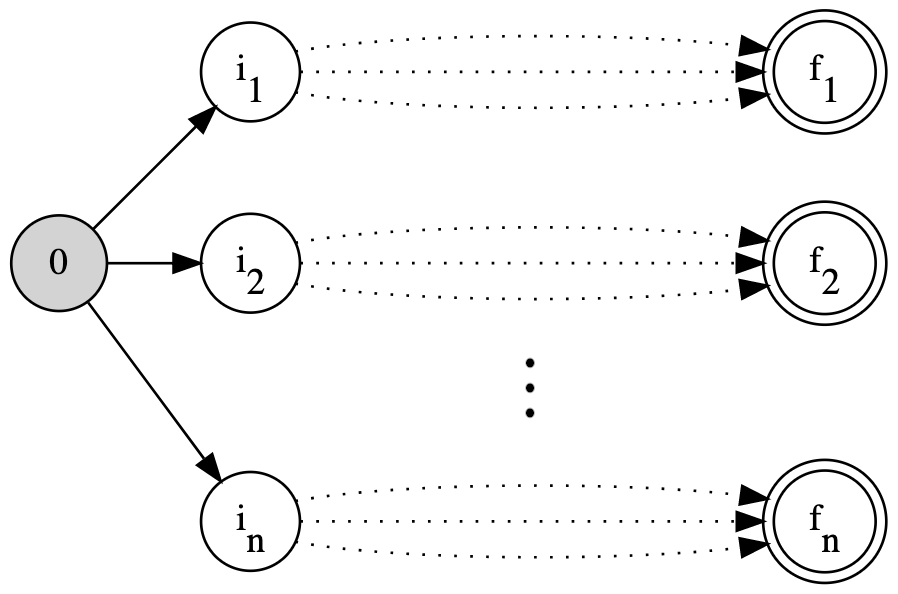
\includegraphics[
		height=5cm,
		keepaspectratio,
	  ]{img/fa-union.png}
	\caption{Краен автомат, получен от обединението на автоматите от лексическа граматика с n на брой правила.}
	\label{fig:FaUnion}
\end{figure}

\begin{example}
	Нека разгледаме следната спецификация:
	\begin{figure}[!htb]
		\begin{center}
			\begin{tabular}{ |l|l| } 
			\hline
			Token & Expression \\
			\hline
			Id & \verb/[a-zA-Z_][a-zA-Z0-9_]*/ \\
			Number & \verb/[0-9]+(\.[0-9]+)?/ \\
			Boolean & \verb/true|false/ \\
			Operator & \verb/=|==|!=|<|<=|>|>=/ \\
			If & \verb/if/ \\
			Else & \verb/else/ \\
			Return & \verb/return/ \\
			BraceOpen & \verb/{/ \\
			BraceClose & \verb/}/\\
			WS & \verb/[ \t\r\n]+/ \\
			\hline
			\end{tabular}
		\end{center}
		\label{fig:Lexgr1}
		\caption{Лексическа граматика}
	\end{figure}

	\noindent Входният текст \emph{"num\textunderscore1=90.4"}, се разбива на следните лексеми: \\ (\emph{num\textunderscore1}, \textbf{Id}), (\emph{=}, \textbf{Operator}), (\emph{90.4}, \textbf{Number}).

	\noindent Друг пример е думата \emph{"if valid==true return 0"}, за която получаваме: \\ (\emph{if}, \textbf{If}), (\emph{' '}, \textbf{WS}), (\emph{valid}, \textbf{Id}), (\emph{==}, \textbf{Operator}), (\emph{true}, \textbf{Boolean}), (\emph{' '}, \textbf{WS}), \\ (\emph{return}, \textbf{Return}), (\emph{' '}, \textbf{WS}), (\emph{0}, \textbf{Number}).

	Всяко правило се представя чрез краен автомат, като на пример този за "Boolean" е изобразен на Фигура \ref{fig:Fa1}.

	\begin{figure}[!htb]
		\centering
		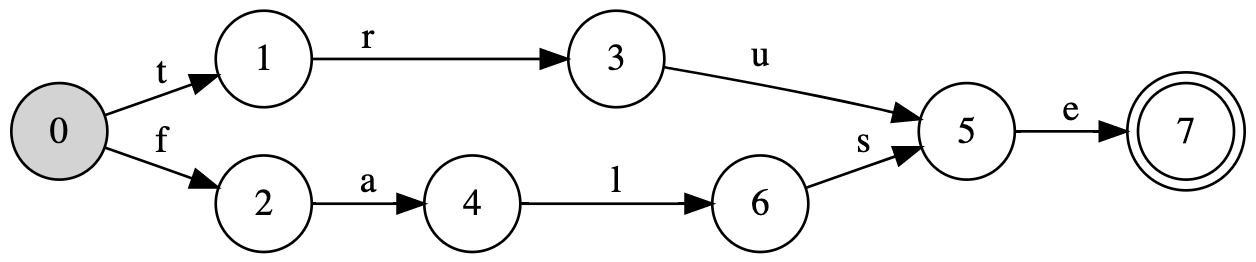
\includegraphics[
			width=12cm,
			keepaspectratio,
	  	]{img/fa1.png}
		\caption{Краен автомат разпознаващ думите \emph{true} или \emph{false}}
		\label{fig:Fa1}
	\end{figure}

	След като автоматите за всяко правило са построени, следващата стъпка е да се обединят в единствен краен автомат (Фигура \ref{fig:Fa3}), който се симулира по време на сканирането на входния текст.

	\begin{figure}[!htb]
		\centering
		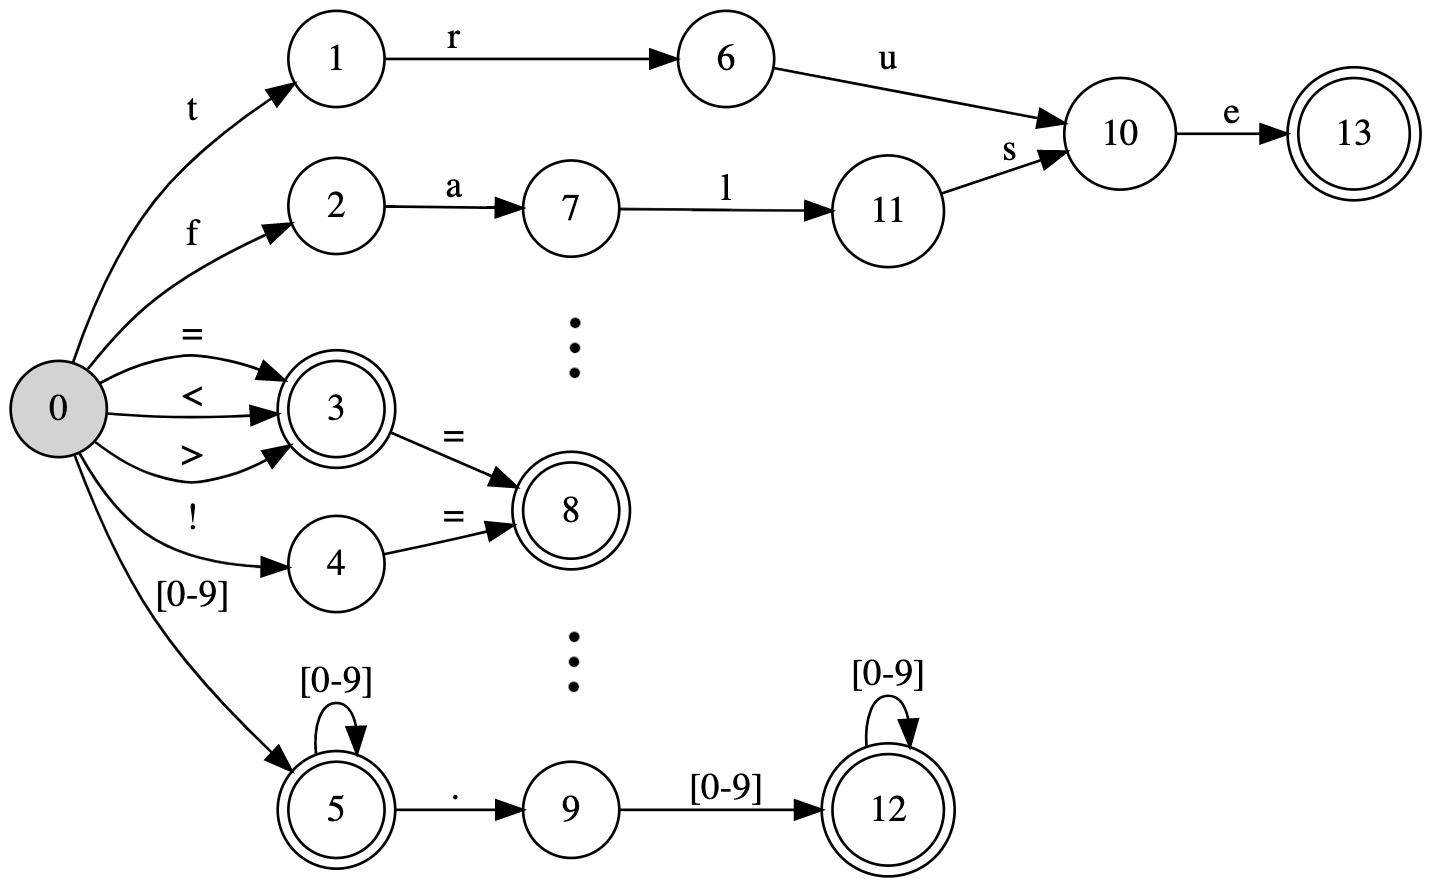
\includegraphics[
			width=16cm,
			height=8cm,
			keepaspectratio,
	  	]{img/fa3.png}
		\caption{Краен автомат, получен от обединението на автоматите от лексическата граматика. За яснота са изобразени само Boolean, Operator и Number.}
		\label{fig:Fa3}
	\end{figure}
	Нека разгледаме входния текст \emph{"1 > 0.99 == true"}. Преди да започнем да го четем, авоматът се намира в началното си състояние 0. Четем \emph{'1'} и преминаваме в състояние 5. Следващият символ е \emph{'>'}, за който няма преход. Намираме се във финално състояние на автомата на лексемата Number, съответно извеждаме (\emph{1}, \textbf{Number}) и се връщаме в началното състояние. Аналогично от 0 имаме преход с \emph{'>'}, който води до състояние 3, което е финално. Няма преход от 3 на \emph{'0'}, съответно извеждаме (\emph{>}, \textbf{Operator}) и се връщаме в 0. Прочитайки \emph{'0'}, автоматът преминава в състояние 5, което е финално, но следващият символ е \emph{'.'}, така че можем да продължим със симулацията като стигаме до състояние 12 и извеждаме (\emph{'0.99'}, \textbf{Number}). Аналогично по пътя 0,3,8 ще изведем (\emph{'=='}, \textbf{Operator}) и в последствие по 0,1,6,10,13 ще изведем (\emph{'true'}, \textbf{Boolean}), като с това сме изчерпали символите в тескта и процедурата приключва.
\end{example}

В определени случаи този подход може да се окаже неефективен. Нека разгледаме следния пример.

\begin{figure}[!htb]
	\begin{center}
		\begin{tabular}{ |l|l| } 
		\hline
		Token & Expression \\
		\hline
		A & \verb/а/ \\
		B & \verb/a+b/ \\
		\hline
		\end{tabular}
	\end{center}
	\centering
	\begingroup
		\tikzset{every picture/.style={scale=0.75}}%
		% Start of code
% \begin{tikzpicture}[anchor=mid,>=latex',line join=bevel,]
\begin{tikzpicture}[>=latex',line join=bevel,]
  \pgfsetlinewidth{1bp}
%%
\pgfsetcolor{black}
  % Edge: 0 -> 1
  \draw [->] (34.057bp,72.693bp) .. controls (44.705bp,78.84bp) and (59.198bp,87.207bp)  .. (80.188bp,99.325bp);
  \definecolor{strokecol}{rgb}{0.0,0.0,0.0};
  \pgfsetstrokecolor{strokecol}
  \draw (57.107bp,94.0bp) node {a};
  % Edge: 0 -> 3
  \draw [->] (34.057bp,55.702bp) .. controls (44.705bp,49.835bp) and (59.198bp,41.848bp)  .. (80.188bp,30.281bp);
  \draw (57.107bp,51.0bp) node {a};
  % Edge: 1 -> 2
  \draw [->] (114.39bp,108.0bp) .. controls (123.82bp,108.0bp) and (135.81bp,108.0bp)  .. (157.02bp,108.0bp);
  \draw (135.71bp,115.0bp) node {a};
  % Edge: 3 -> 3
  \draw [->] (89.48bp,39.037bp) .. controls (88.106bp,48.858bp) and (90.351bp,58.0bp)  .. (96.214bp,58.0bp) .. controls (99.878bp,58.0bp) and (102.13bp,54.429bp)  .. (102.95bp,39.037bp);
  \draw (96.214bp,65.0bp) node {a};
  % Edge: 3 -> 4
  \draw [->] (114.39bp,22.0bp) .. controls (123.82bp,22.0bp) and (135.81bp,22.0bp)  .. (157.02bp,22.0bp);
  \draw (135.71bp,29.0bp) node {b};
  % Node: 0
\begin{scope}
  \definecolor{strokecol}{rgb}{0.0,0.0,0.0};
  \pgfsetstrokecolor{strokecol}
  \definecolor{fillcol}{rgb}{0.83,0.83,0.83};
  \pgfsetfillcolor{fillcol}
  \filldraw [opacity=1] (18.0bp,64.0bp) ellipse (18.0bp and 18.0bp);
  \draw (18.0bp,64.0bp) node {0};
\end{scope}
  % Node: 1
\begin{scope}
  \definecolor{strokecol}{rgb}{0.0,0.0,0.0};
  \pgfsetstrokecolor{strokecol}
  \draw (96.21bp,108.0bp) ellipse (18.0bp and 18.0bp);
  \draw (96.214bp,108.0bp) node {1};
\end{scope}
  % Node: 3
\begin{scope}
  \definecolor{strokecol}{rgb}{0.0,0.0,0.0};
  \pgfsetstrokecolor{strokecol}
  \draw (96.21bp,22.0bp) ellipse (18.0bp and 18.0bp);
  \draw (96.214bp,22.0bp) node {3};
\end{scope}
  % Node: 2
\begin{scope}
  \definecolor{strokecol}{rgb}{0.0,0.0,0.0};
  \pgfsetstrokecolor{strokecol}
  \draw (179.21bp,108.0bp) ellipse (18.0bp and 18.0bp);
  \draw (179.21bp,108.0bp) ellipse (22.0bp and 22.0bp);
  \draw (179.21bp,108.0bp) node {2};
\end{scope}
  % Node: 4
\begin{scope}
  \definecolor{strokecol}{rgb}{0.0,0.0,0.0};
  \pgfsetstrokecolor{strokecol}
  \draw (179.21bp,22.0bp) ellipse (18.0bp and 18.0bp);
  \draw (179.21bp,22.0bp) ellipse (22.0bp and 22.0bp);
  \draw (179.21bp,22.0bp) node {4};
\end{scope}
%
\end{tikzpicture}
% End of code
	\endgroup
	\label{fig:Lexgr2}
	\caption{Лексическа граматика и построеният по нея краен автомат.}
\end{figure}

\begin{example}
	Граматиката на Фигура \ref{fig:Lexgr2} съдържа две правила. Правило \textbf{A} представлява единствено думата \emph{"a"}. Правило \textbf{B} обхваща думите, съдържащи \emph{'a'} поне веднъж, които завършват с \emph{'b'} като на пример \emph{"ab", "aab", "aaab"} и т.н. Входният текст \emph{"aabaa"} се разбива на следните лексеми: (\emph{'aab'}, \textbf{B}), (\emph{'a'}, \textbf{A}), (\emph{'a'}, \textbf{A}).

	Нека разгледаме случая, в който сканираме текста \emph{"aaaaaaaaаа"}, състоящ се от десет еднакви лексеми - (\emph{'a'}, \textbf{A}). Очевидно, за да изведем \textbf{А} е необходимо да сканираме текста до самия му край, за да се уверим, че не съществува \emph{'b'}. Това се случва за всеки изведен тоукън, което води до неоптимална сложност на процедурата от \( \mathcal{O}(n^2) \).
\end{example}

Лексическият анализ чрез бимашина се справя с този проблем като сканирането на текста се случва едновременно от ляво на дясно и от дясно на ляво, с което се гарантира линейно време на изпълнение. Целта на тази работа е да се представи конструкция на такава бимашина по зададена лексическа граматика и алгоритъм за осъществяване на лексическия анализ.

\pagebreak
\section{Основни дефиниции}

\subsection{Крайни автомати}

\begin{definition}
	\emph{Краен автомат} дефинираме като петорка \( \mathcal{A} = \langle \Sigma, Q, I, F, \Delta \rangle \), където

	\begin{itemize}
		\item \( \Sigma \) е \emph{крайна азбука от символи}
		\item \( Q \) е \emph{крайно множество от състояния}
		\item \( I \subseteq Q \) е \emph{множество от начални състояния}
		\item \( F \subseteq Q \) е \emph{множество от финални състояния}
		\item \( \Delta \subseteq Q \times \Sigma \times Q \) е \emph{релация на прехода}
	\end{itemize}
 
	Тройки от вида \( \langle q_1, m, q_2 \rangle \in \Delta \) наричаме \emph{преходи} и казваме, че започва състояние \( q_1 \), има етикет \( m \) и завършва в състояние \( q_2 \). Алтернативно, тези преходи обозначаваме като \( q_1 \to^m q_2 \).
\end{definition}

\begin{definition}  
	Нека \( \mathcal{A} \) е краен автомат. \emph{Разширена релация на прехода} \( \Delta^* \subseteq Q \times \Sigma^* \times Q \) дефинираме индуктивно:

	\begin{itemize}
		\item \( \langle q, \epsilon, q \rangle \in \Delta^* \) за всяко \( q \in Q \)
		\item \( \langle q_1, wa, q_2 \rangle \in \Delta^* \) за всяко \( q_1, q_2, q \in Q \), \( a \in \Sigma, w \in \Sigma^* \), ако \( \langle q_1, w, q \rangle \in \Delta^* \) и \( \langle q, a, q_2 \rangle \in \Delta \)
	\end{itemize}
\end{definition}

\begin{definition} 
	Нека \( \mathcal{A} = \langle \Sigma, Q, I, F, \Delta \rangle \) е краен автомат. \emph{Път} в \( \mathcal{A} \) наричаме крайна редица от преходи с дължина \( k > 0 \) 
	\[ \pi = q_0 \to^{a_1} q_1 \to^{a_2} \ldots \to^{a_k} q_k \] 
	където \( \langle q_{i-1}, a_i, q_i \rangle \in \Delta \) за \( i = 1 \ldots k \). Казваме, че \emph{пътят} започва от състояние \( q_0 \) и завършва в състояние \( q_k \). Елементите \( q_0,q_1, \ldots ,q_k \) наричаме \emph{състояния на пътя}, а думата \( w = a_1 a_2 \ldots a_k \) наричаме \emph{етикет на пътя}. \newline \emph{Успешен път} в автомата е \emph{път}, който започва от начално състояние и завършва във финално състояние.
\end{definition}

\begin{figure}[!htb]
	\centering
	% Start of code
% \begin{tikzpicture}[anchor=mid,>=latex',line join=bevel,]
\begin{tikzpicture}[>=latex',line join=bevel,]
  \pgfsetlinewidth{1bp}
%%
\pgfsetcolor{black}
  % Edge: 0 -> 1
  \draw [->] (41.38bp,33.346bp) .. controls (53.024bp,40.533bp) and (68.186bp,49.893bp)  .. (89.207bp,62.868bp);
  \definecolor{strokecol}{rgb}{0.0,0.0,0.0};
  \pgfsetstrokecolor{strokecol}
  \draw (65.5bp,56.0bp) node {b};
  % Edge: 0 -> 2
  \draw [->] (44.085bp,23.735bp) .. controls (64.334bp,25.44bp) and (95.778bp,28.188bp)  .. (123.0bp,31.0bp) .. controls (133.76bp,32.112bp) and (145.59bp,33.464bp)  .. (165.94bp,35.889bp);
  \draw (105.0bp,38.0bp) node {\(\epsilon\)};
  % Edge: 1 -> 1
  \draw [->] (98.266bp,89.037bp) .. controls (96.892bp,98.858bp) and (99.137bp,108.0bp)  .. (105.0bp,108.0bp) .. controls (108.66bp,108.0bp) and (110.92bp,104.43bp)  .. (111.73bp,89.037bp);
  \draw (105.0bp,115.0bp) node {a};
  % Edge: 1 -> 2
  \draw [->] (122.93bp,73.777bp) .. controls (130.82bp,73.967bp) and (140.18bp,73.252bp)  .. (148.0bp,70.0bp) .. controls (154.19bp,67.427bp) and (159.98bp,63.257bp)  .. (172.2bp,51.623bp);
  \draw (144.5bp,79.0bp) node {a};
  % Edge: 1 -> 2
  \draw [->] (120.65bp,62.769bp) .. controls (126.79bp,59.127bp) and (134.1bp,55.085bp)  .. (141.0bp,52.0bp) .. controls (145.96bp,49.782bp) and (151.38bp,47.722bp)  .. (166.36bp,42.716bp);
  \draw (144.5bp,59.0bp) node {b};
  % Edge: 2 -> 0
  \draw [->] (168.41bp,28.627bp) .. controls (156.67bp,21.673bp) and (139.47bp,12.77bp)  .. (123.0bp,9.0bp) .. controls (99.748bp,3.6755bp) and (72.92bp,7.7011bp)  .. (43.121bp,15.249bp);
  \draw (105.0bp,16.0bp) node {a};
  % Node: 0
\begin{scope}
  \definecolor{strokecol}{rgb}{0.0,0.0,0.0};
  \pgfsetstrokecolor{strokecol}
  \definecolor{fillcol}{rgb}{0.83,0.83,0.83};
  \pgfsetfillcolor{fillcol}
  \filldraw [opacity=1] (22.0bp,22.0bp) ellipse (18.0bp and 18.0bp);
  \draw (22.0bp,22.0bp) ellipse (22.0bp and 22.0bp);
  \draw (22.0bp,22.0bp) node {0};
\end{scope}
  % Node: 1
\begin{scope}
  \definecolor{strokecol}{rgb}{0.0,0.0,0.0};
  \pgfsetstrokecolor{strokecol}
  \draw (105.0bp,72.0bp) ellipse (18.0bp and 18.0bp);
  \draw (105.0bp,72.0bp) node {1};
\end{scope}
  % Node: 2
\begin{scope}
  \definecolor{strokecol}{rgb}{0.0,0.0,0.0};
  \pgfsetstrokecolor{strokecol}
  \draw (184.0bp,38.0bp) ellipse (18.0bp and 18.0bp);
  \draw (184.0bp,38.0bp) node {2};
\end{scope}
%
\end{tikzpicture}
% End of code

	\caption{Недетерминиран краен автомат}
	\label{fig:Nfa}
\end{figure}

\begin{example}
	Нека е зададена азбука \( \Sigma = \{ a,b,\epsilon \} \) и автомат \( \mathcal{A} \) над \( \Sigma \) със състояния \( Q = \{ 0, 1, 2 \} \), начални \( I = \{ 0 \} \), финални \( F = \{ 0 \} \) и релация на прехода 
	\[ \Delta = \{ \langle 0, b, 1 \rangle, \langle 0, \epsilon, 2 \rangle, \langle 1, a, 1 \rangle, \langle 1, a, 2 \rangle \, \langle 1, b, 2 \rangle, \langle 2, a, 0 \rangle \} \]
	\( \mathcal{A} \) е изобразен на Фигура \ref{fig:Nfa}. \( 0 \to^{b} 1 \to^{a} 1 \to^{b} 2 \to^{a} 0 \) е успешен път, разпознавайки думата \emph{baba}.
\end{example}

\begin{definition} 
	Нека \( \mathcal{A} \) е краен автомат. Множеството от етикети на всички успещни пътища в \( \mathcal{A} \) наричаме \emph{език на \( \mathcal{A} \)} и обозначаваме като \( L(\mathcal{A}) \). \[ L(\mathcal{A}) = \{ w \in \Sigma^* \mid \exists i \in I, f \in F : \langle i, w, f \rangle \in \Delta^* \} \]
\end{definition}

\begin{definition} 
	Нека \( \mathcal{A}_1 \) и \( \mathcal{A}_2 \) са крайни автомати. Казваме, че \( \mathcal{A}_1 \) е еквивалентен на \( \mathcal{A}_2 \) (\( \mathcal{A}_1 \equiv \mathcal{A}_2 \)), ако езиците им съвпадат (\( L(\mathcal{A}_1) = L(\mathcal{A}_2) \))
\end{definition}

\begin{definition}
	Нека \( \mathcal{A} = \langle \Sigma, Q, I, F, \Delta \rangle \) е краен автомат. Автоматът \(\mathcal{A'} = \langle Q, F, I, \Delta' \), където \( \Delta' = \{ \langle q, a, p \rangle \mid \langle p, a, q \rangle \in \Delta \} \) наричаме \emph{огледален} na \(\mathcal{A}\). За всяка дума \( w = w_1w_2 \dots w_k \in L(\mathcal{A}) \) е в сила \( w' = w_k \dots w_2w_1 \in L(\mathcal{A'}) \).
\end{definition}

\begin{definition}
	Kраен автомат \( \mathcal{A} = \langle \Sigma, Q, I, F, \Delta \rangle \) е \emph{детерминиран}, ако:

	\begin{itemize}
		\item \( \mathcal{A} \) има единствено начално състояние \(I = \{q_0\}\).
		\item За всяко \( q_1 \in Q \) и символ \( a \in \Sigma \), съществува не повече от едно \( q_2 \in Q \), такова че \( \langle q_1, a, q_2 \rangle \in \Delta \).
	\end{itemize} 

	\noindent Иначе казано, релацията на прехода може да се представи като частична функция \( \delta: Q \times \Sigma \to Q \) и \emph{детерминираните автомати} можем преставим в следния вид \[ \mathcal{A}_D = \langle \Sigma, Q, q_0, F, \delta \rangle \]

	Предимството на \emph{детерминираните автомати} се изразява в това, че могат да разпознават дали дума \( w \) принадлежи на езика на автомата \( L(\mathcal{A}_D) \) за линейно време спрямо дължината ѝ - \( O(|w|) \), но в определени случаи могат да имат експоненциален брой състояния спрямо еквивалентният им недетерминиран автомат.
\end{definition}

\begin{figure}[!htb]
	\centering
	% Start of code
% \begin{tikzpicture}[anchor=mid,>=latex',line join=bevel,]
\begin{tikzpicture}[>=latex',line join=bevel,]
  \pgfsetlinewidth{1bp}
%%
\pgfsetcolor{black}
  % Edge: 0 -> 0
  \draw [->] (14.317bp,42.991bp) .. controls (13.369bp,53.087bp) and (15.93bp,62.0bp)  .. (22.0bp,62.0bp) .. controls (25.889bp,62.0bp) and (28.337bp,58.342bp)  .. (29.683bp,42.991bp);
  \definecolor{strokecol}{rgb}{0.0,0.0,0.0};
  \pgfsetstrokecolor{strokecol}
  \draw (22.0bp,69.0bp) node {a};
  % Edge: 0 -> 1
  \draw [->] (43.022bp,29.416bp) .. controls (53.675bp,33.361bp) and (66.893bp,38.257bp)  .. (87.741bp,45.978bp);
  \draw (65.5bp,46.0bp) node {b};
  % Edge: 1 -> 2
  \draw [->] (119.63bp,62.906bp) .. controls (131.01bp,72.014bp) and (147.44bp,85.165bp)  .. (168.71bp,102.19bp);
  \draw (144.11bp,91.0bp) node {a};
  % Edge: 1 -> 3
  \draw [->] (123.04bp,52.0bp) .. controls (150.43bp,52.0bp) and (204.51bp,52.0bp)  .. (247.82bp,52.0bp);
  \draw (183.21bp,59.0bp) node {b};
  % Edge: 2 -> 3
  \draw [->] (197.95bp,102.65bp) .. controls (210.29bp,93.363bp) and (228.62bp,79.56bp)  .. (251.41bp,62.399bp);
  \draw (222.71bp,93.0bp) node {b};
  % Edge: 2 -> 4
  \draw [->] (197.25bp,124.43bp) .. controls (203.47bp,129.19bp) and (211.28bp,134.25bp)  .. (219.21bp,137.0bp) .. controls (223.88bp,138.62bp) and (228.98bp,139.63bp)  .. (244.14bp,140.96bp);
  \draw (222.71bp,145.0bp) node {a};
  % Edge: 3 -> 0
  \draw [->] (248.27bp,47.884bp) .. controls (221.74bp,41.645bp) and (168.72bp,29.994bp)  .. (123.0bp,25.0bp) .. controls (100.13bp,22.501bp) and (74.15bp,21.785bp)  .. (44.136bp,21.67bp);
  \draw (144.11bp,36.0bp) node {a};
  % Edge: 4 -> 2
  \draw [->] (247.16bp,128.57bp) .. controls (240.77bp,124.99bp) and (233.37bp,121.36bp)  .. (226.21bp,119.0bp) .. controls (221.48bp,117.44bp) and (216.31bp,116.29bp)  .. (201.28bp,114.07bp);
  \draw (222.71bp,126.0bp) node {b};
  % Edge: 4 -> 4
  \draw [->] (258.53bp,160.99bp) .. controls (257.58bp,171.09bp) and (260.14bp,180.0bp)  .. (266.21bp,180.0bp) .. controls (270.1bp,180.0bp) and (272.55bp,176.34bp)  .. (273.9bp,160.99bp);
  \draw (266.21bp,187.0bp) node {a};
  % Node: 0
\begin{scope}
  \definecolor{strokecol}{rgb}{0.0,0.0,0.0};
  \pgfsetstrokecolor{strokecol}
  \definecolor{fillcol}{rgb}{0.83,0.83,0.83};
  \pgfsetfillcolor{fillcol}
  \filldraw [opacity=1] (22.0bp,22.0bp) ellipse (18.0bp and 18.0bp);
  \draw (22.0bp,22.0bp) ellipse (22.0bp and 22.0bp);
  \draw (22.0bp,22.0bp) node {0};
\end{scope}
  % Node: 1
\begin{scope}
  \definecolor{strokecol}{rgb}{0.0,0.0,0.0};
  \pgfsetstrokecolor{strokecol}
  \draw (105.0bp,52.0bp) ellipse (18.0bp and 18.0bp);
  \draw (105.0bp,52.0bp) node {1};
\end{scope}
  % Node: 2
\begin{scope}
  \definecolor{strokecol}{rgb}{0.0,0.0,0.0};
  \pgfsetstrokecolor{strokecol}
  \draw (183.21bp,113.0bp) ellipse (18.0bp and 18.0bp);
  \draw (183.21bp,113.0bp) node {2};
\end{scope}
  % Node: 3
\begin{scope}
  \definecolor{strokecol}{rgb}{0.0,0.0,0.0};
  \pgfsetstrokecolor{strokecol}
  \draw (266.21bp,52.0bp) ellipse (18.0bp and 18.0bp);
  \draw (266.21bp,52.0bp) node {3};
\end{scope}
  % Node: 4
\begin{scope}
  \definecolor{strokecol}{rgb}{0.0,0.0,0.0};
  \pgfsetstrokecolor{strokecol}
  \draw (266.21bp,140.0bp) ellipse (18.0bp and 18.0bp);
  \draw (266.21bp,140.0bp) ellipse (22.0bp and 22.0bp);
  \draw (266.21bp,140.0bp) node {4};
\end{scope}
%
\end{tikzpicture}
% End of code

	\caption{Детерминиран краен автомат}
\end{figure}

\begin{definition}
	Нека \( \mathcal{A}_D = \langle \Sigma, Q, q_0, F, \delta \rangle \) е \emph{детерминиран краен автомат}. \emph{Разширена функция на прехода} \( \delta^*: Q \times \Sigma^* \to Q \) дефинираме индуктивно:

	\begin{itemize}
		\item \( \delta^*(q, \epsilon) = q \)
		\item \( \delta^*(q, aw) = \delta^*(\delta(q, a), w) \), където \( a \in \Sigma, w \in \Sigma^* \)
	\end{itemize}
\end{definition}

\begin{theorem}
	За всеки краен автомат \(\mathcal{A} = \langle \Sigma, Q, I, F, \Delta \rangle \), съществува еквивалентен на него, детерминиран краен автомат \( \mathcal{A}_D \), където \( L(\mathcal{A}) = L(\mathcal{A}_D) \).
	\begin{proof}
		Нека \( \mathcal{A} \) е краен автомат, на който сме премахнали \( \epsilon \)-преходите. Строим \emph{детерминиран краен автомат} \( \mathcal{A}_D = \langle \Sigma, 2^Q, I, F_D, \delta \rangle \), където:
		\begin{itemize}
			\item \( F_D = \{ S \in 2^Q \mid S \cap F \neq \emptyset \} \)
			\item \( \delta(S,a) = \{ q \in Q \mid \exists p \in S : \langle p, a, q \rangle \in \Delta \} \)
		\end{itemize}
		С индукция по дължината на \( w \), ще покажем, че за произволна дума \( w \in \Sigma^* \) твръденията \( \exists i \in I: \langle i, w, p \rangle \in \Delta^* \) и \( p \in \delta^*(I, w)\) са еквивалентни:
		\begin{itemize}
			\item \emph{База}: за \( |w| = 0 \) имаме \( w = \epsilon \). Тогава \( \exists i \in I: \langle  i, \epsilon, i \rangle \in \Delta^* \). Тъй като \( \mathcal{A} \) няма \( \epsilon \)-преходи, то \( \delta^*(I, \epsilon) = I \).
			
			\item \emph{Индукция}: \( w = w'a, a \in \Sigma, |w| = |w'| + 1 \). \newline
			\( (\Rightarrow) \) Нека допуснем, че \( \exists i \in I \), така че \( \langle i, w'a, p \rangle \in \Delta^* \), което значи, че \( \exists p' \in Q: \langle p', a, p \rangle \in \Delta \). По индуктивното предположение знаем, че и \( p' \in \delta^*(I, w') \) и от дефиницията на \( \delta \) следва, че \( p \in \delta(\delta^*(I, w'), a) \). \newline
			\( (\Leftarrow) \) Нека допуснем, че \( p \in \delta^*(I, w'a) \). Тогава \( \exists p': p' \in \delta^*(I, w') \). От индуктивното предположение знаем, че \( \langle i, w', p' \rangle \in \Delta^* \) и от дефинициите на \( \delta  \) и \( \Delta \) следва, че \( \langle p', a, p \rangle \in \Delta \), от където следва, че \( \exists i \in I: \langle i, w'a, p \rangle \in \Delta^* \).
		\end{itemize}
		Така можем да заключим, че за всяка дума \( w \in L(\mathcal{A}) \), \( \exists i \in I, \exists f \in F : \langle i, w, f \rangle \in \Delta^* \) е изпълнено, че \( \delta^*(I, w) \in F_D \), следователно \( w \in L(\mathcal{A}_D) \) и \( L(\mathcal{A}) = L(\mathcal{A}_D) \).
	\end{proof}
\end{theorem}

\subsection{Крайни преобразуватели}

\begin{definition}
	\emph{Краен преобразувател} дефинираме като петорка \( \mathcal{T} = \langle \Sigma_1^* \times \Sigma_2^*, Q, I, F, \Delta \rangle \), където

	\begin{itemize}
		\item \( \Sigma_1, \Sigma_2 \) са \emph{крайни азбуки от символи}
		\item \( Q \) е \emph{крайно множество от състояния}
		\item \( I \subseteq Q \) е \emph{множество от начални състояния}
		\item \( F \subseteq Q \) е \emph{множество от финални състояния}
		\item \( \Delta \subseteq Q \times (\Sigma_1^* \times \Sigma_2^*) \times Q \) е \emph{релация на прехода}
	\end{itemize}
 
	Тройки от вида \( \langle q_1, \langle w, m \rangle, q_2 \rangle \in \Delta \) наричаме \emph{преходи} и казваме, че започва състояние \( q_1 \), има етикет по горната лента \( w \) и по долната лента \( m \) и завършва в състояние \( q_2 \). Алтернативно, тези преходи обозначаваме като \( q_1 \to^w_m q_2 \).
\end{definition}

\begin{definition} 
	Нека \( \mathcal{T} = \langle \Sigma_1^* \times \Sigma_2^*, Q, I, F, \Delta \rangle \) е краен преобразувател. \emph{Път} в \( \mathcal{T} \) наричаме крайна редица от преходи с дължина \( k > 0 \) 
	\[ \pi = q_0 \to^{w_1}_{m_1} q_1 \to^{w_2}_{m_2} \ldots \to^{w_k}_{m_k}  q_k \] 
	където \( \langle q_{i-1}, \langle w_i, m_i \rangle, q_i \rangle \in \Delta \) за \( i = 1 \ldots k \). Казваме, че \emph{пътят} започва от състояние \( q_0 \) и завършва в състояние \( q_k \). Елементите \( q_0,q_1, \ldots ,q_k \) наричаме \emph{състояния на пътя}, а думата \( w = w_1 w_2 \ldots w_k \) наричаме \emph{входна дума} на пътя, а \( m = m_1 m_2 \ldots m_k \) е \emph{изходна дума} на пътя. \newline \emph{Успешен път} в преобразувателя започва от начално състояние и завършва във финално състояние.
\end{definition}

\begin{figure}[!htb]
	\centering
	% Start of code
% \begin{tikzpicture}[anchor=mid,>=latex',line join=bevel,]
\begin{tikzpicture}[>=latex',line join=bevel,]
  \pgfsetlinewidth{1bp}
%%
\pgfsetcolor{black}
  % Edge: 0 -> 1
  \draw [->] (36.835bp,66.461bp) .. controls (43.628bp,73.272bp) and (52.411bp,80.407bp)  .. (62.0bp,84.0bp) .. controls (70.197bp,87.071bp) and (79.618bp,87.58bp)  .. (98.159bp,85.873bp);
  \definecolor{strokecol}{rgb}{0.0,0.0,0.0};
  \pgfsetstrokecolor{strokecol}
  \draw (70.945bp,94.0bp) node {a/d};
  % Edge: 0 -> 2
  \draw [->] (42.234bp,41.004bp) .. controls (48.469bp,38.253bp) and (55.463bp,35.34bp)  .. (62.0bp,33.0bp) .. controls (70.433bp,29.982bp) and (79.79bp,27.161bp)  .. (98.033bp,22.16bp);
  \draw (70.945bp,40.0bp) node {b/d};
  % Edge: 1 -> 0
  \draw [->] (99.425bp,74.306bp) .. controls (93.413bp,71.481bp) and (86.413bp,68.392bp)  .. (79.89bp,66.0bp) .. controls (71.374bp,62.877bp) and (61.955bp,60.003bp)  .. (43.517bp,54.95bp);
  \draw (70.945bp,73.0bp) node {b/\(\epsilon\)};
  % Edge: 2 -> 0
  \draw [->] (99.067bp,10.797bp) .. controls (88.259bp,6.9443bp) and (73.813bp,3.9331bp)  .. (62.0bp,9.0bp) .. controls (54.255bp,12.322bp) and (47.322bp,18.021bp)  .. (34.816bp,31.943bp);
  \draw (70.945bp,16.0bp) node {c/\(\epsilon\)};
  % Node: 0
\begin{scope}
  \definecolor{strokecol}{rgb}{0.0,0.0,0.0};
  \pgfsetstrokecolor{strokecol}
  \definecolor{fillcol}{rgb}{0.83,0.83,0.83};
  \pgfsetfillcolor{fillcol}
  \filldraw [opacity=1] (22.0bp,50.0bp) ellipse (18.0bp and 18.0bp);
  \draw (22.0bp,50.0bp) ellipse (22.0bp and 22.0bp);
  \draw (22.0bp,50.0bp) node {0};
\end{scope}
  % Node: 1
\begin{scope}
  \definecolor{strokecol}{rgb}{0.0,0.0,0.0};
  \pgfsetstrokecolor{strokecol}
  \draw (115.89bp,82.0bp) ellipse (18.0bp and 18.0bp);
  \draw (115.89bp,82.0bp) node {1};
\end{scope}
  % Node: 2
\begin{scope}
  \definecolor{strokecol}{rgb}{0.0,0.0,0.0};
  \pgfsetstrokecolor{strokecol}
  \draw (115.89bp,18.0bp) ellipse (18.0bp and 18.0bp);
  \draw (115.89bp,18.0bp) node {2};
\end{scope}
%
\end{tikzpicture}
% End of code

	\caption{Краен преобразувател}
	\label{fig:Fst}
\end{figure}

\begin{example}
	Нека са зададени азбуки \( \Sigma_1 = \{ a,b,c \}, \Sigma_2 = \{ d,\epsilon \} \) и преобразувател \( \mathcal{T} \) над \( \Sigma_1 \times \Sigma_2 \) със състояния \( Q = \{ 0, 1, 2 \} \), начални \( I = \{ 0 \} \), финални \( F = \{ 0 \} \) и релация на прехода \( \Delta = \{ \langle 0, \langle a, d \rangle, 1 \rangle, \langle 1, \langle b, \epsilon \rangle, 0 \rangle, \langle 0, \langle b, d \rangle, 2 \rangle, \langle 2, \langle c, \epsilon \rangle, 0 \rangle \} \). \newline
	\( \mathcal{T} \) е изобразен на Фигура \ref{fig:Fst}. \newline
	\( 0 \to^{b}_{d} 2 \to^{c}_{\epsilon} 0 \to^{a}_{d} 1 \to^{b}_{\epsilon} 0 \) е успешен път, превеждайки думата \emph{bcab} в \emph{dd}.
\end{example}

\begin{definition}
	Нека \( \mathcal{T} = \langle \Sigma_1^* \times \Sigma_2^*, Q, I, F, \Delta \rangle \) е краен преобразувател. \emph{Подлежащ автомат} на \( \mathcal{T} \) дефинираме като \( \mathcal{A} = \langle \Sigma, Q, I, F, \Delta' \rangle \), където \( \Delta' = \{ \langle p, w, q \rangle \mid \langle p, \langle w, m \rangle, q \rangle \in \Delta \}\)
\end{definition}

\subsection{Регулярни езици и релации}

\begin{definition} 
	\emph{Регулярен език} е множество от думи над крайна азбука \( \Sigma \), което дефинираме индуктивно:
	\begin{itemize}
		\item \( \emptyset \) е регулярен език.
		\item ако \( a \in \Sigma \), то \( \{ a \} \) е регулярен език.
		\item ако \( L_1, L_2 \subseteq \Sigma^* \) са регулярни езици, то 
		\begin{itemize}
			\item \( L_1 \cup L_2 \) (обедниение)
			\item \( L_1 \cdot L_2 = \{ a \cdot b \mid a \in L_1, b \in L_2 \} \) (конкатенация)
			\item \( L_1^* = \bigcup_{i=0}^{\infty}L^i \) (звезда на Клини)
		\end{itemize}
		 са също регулярни езици.
		\item Не съществуват други регулярни езици.
	\end{itemize}
	Регулярните езици са също така \emph{затворени} относно операциите \emph{разлика} (\( L_1 \setminus L_2 \)), \emph{обръщане} (\( L_1^{-1} \)) и \emph{сечение} (\( L_1 \cap L_2 \)).
\end{definition}

\begin{definition} 
	\emph{Двоична регулярна стрингова релация} дефинираме индуктивно като множество от двойки думи над крайни азбуки \( \Sigma_1, \Sigma_2 \):
	\begin{itemize}
		\item \( \emptyset \) е регулярна релация.
		\item Ако \( a \in \Sigma_1 \times \Sigma_2 \), то \( \{ a \} \) е регулярна релация.
		\item Ако \( R_1, R_2 \) са регулярни релации, то:
		\begin{itemize}
			\item \( R_1 \cup R_2 \) (обединение)
			\item \( R_1 \cdot R_2 = \{ a \cdot b \mid a \in R_1, b \in R_2 \} \) (конкатенация)
			\item \( R_1^* = \bigcup_{i=0}^{\infty}R^i \) (звезда на Клини)
		\end{itemize}
		са също регулярни релации.
		\item Не съществуват други регулярни релации.
	\end{itemize}
\end{definition}

\begin{definition}
	Нека \( R_1, R_2, \subseteq \Sigma^* \times \Sigma^* \) са \emph{двоични стрингови релации}. \emph{Конкатенацията} на \( R_1 \) и \( R_2 \) дефинираме както следва
	\[ R_1 \cdot R_2 = \{ \langle u_1 v_1, u_2 v_2 \rangle \mid \langle u_1, u_2 \rangle \in R_1, \langle v_1, v_2 \rangle \in R_2 \} \]
\end{definition}

\begin{definition}
	Нека \( R_1, R_2, \subseteq \Sigma^* \times \Sigma^* \) са \emph{двоични стрингови релации}. \emph{Композицията} на \( R_1 \) и \( R_2 \) дефинираме както следва
	\[ R_1 \circ R_2 = \{ \langle a, c \rangle \mid \exists b \in \Sigma^* : \langle a, b \rangle \in R_1, \langle b, c \rangle \in R_2 \} \]
\end{definition}

\begin{definition} 
	\emph{Регулярен израз} наричаме дума над крайна азбука \( \Sigma \cup \{ (, ), \vert, * \} \)
	\begin{itemize}
		\item \( \epsilon \) е регулярен израз.
		\item Ако \( a \in \Sigma \), то \( a \) е регулярен израз.
		\item Ако \( E_1, E_2 \) са регулярни изрази, то \( E_1 | E_2 \) и \( E_1 E_2 \), \( E_1^* \) също са регулярни изрази.
		\item Не съществуват други регулярни изрази.
	\end{itemize}
	Всеки регулярен израз има сътветстващ регулярен език:
	\begin{itemize}
		\item \( L(\epsilon) = \emptyset \)
		\item \( L(a) = \{ a \}, a \in \Sigma \)
		\item \( L(E_1 | E_2) = L(E_1) \cup L(E_2) \)
		\item \( L(E_1 E_2) = L(E_1) \cdot L(E_2) \)
		\item \( L(E_1^*) = L(E_1)^* \)
	\end{itemize}
\end{definition}

\begin{example}
	\verb/(a|b)*c/ е \emph{регулярен израз}, разпознаващ думите \emph{c, ac, bc, aac, abc, abbc, bababbc ...}
\end{example}

\begin{theorem}{\emph{(Клини)}}
	За всеки регулярен израз \( E \) съществува краен автомат \( \mathcal{A} \), за който \( L(E) = L(\mathcal{A})\).
\end{theorem}

\begin{theorem}
	Всяка двоична регулярна стрингова релация може да се представи, чрез класически краен преобразувател.
\end{theorem}

\begin{example}
	\( R = \{ \langle ab, d \rangle, \langle bc, d \rangle \}^* \) е \emph{регулярна релация}, която е представена чрез крайния преобразувател \(\mathcal{T}\) на Фигура \ref{fig:Fst}. С \emph{dom(R)} бележим домейна на \(R\), който изразяваме чрез \emph{подлежащия автомат} на \( \mathcal{T} \), \( dom(R) =  \{ ab, bc, abab, abbc, bcab \dots \} \). С \emph{range(R)} обозначаваме кодомейна на релацията \( range(R) =  \{ \epsilon, d, dd, ddd, dddd \dots \} \).
\end{example}

\begin{example}
	Нека \(L\) е \emph{регулярен език}. \( Id(L) = \{ \langle w, w \rangle \mid w \in L \}\) е \emph{регулярна релация}.
\end{example}

\begin{definition}
	\emph{Регулярна стрингова функция} наричаме регулярна стрингова релация, която е частична функция. 
\end{definition}

\subsection{Бимашини}

\begin{definition}
	 \emph{Класическа бимашина} дефинираме като тройка \( \mathcal{B} = \langle \mathcal{A}_L, \mathcal{A}_R, \psi \rangle \), където

	\begin{itemize}
		\item \( \mathcal{A}_L = \langle \Sigma, Q_L, s_L, Q_L, \delta_L \rangle \) и \( \mathcal{A}_R = \langle \Sigma, Q_R, s_R, Q_R, \delta_R \rangle \) са \emph{детерминирани крайни автомати} и ги наричаме съответно \emph{ляв и десен автомат} на бимашината. Всички състояния на тези автомати са финални.
		\item \( \psi:(Q_L \times \Sigma \times Q_R) \to \Sigma^* \) e частична функция, която наричаме \emph{изходна функция}.
	\end{itemize}
\end{definition}

\begin{definition}
	Нека \( \mathcal{B} = \langle \mathcal{A}_L, \mathcal{A}_R, \psi \rangle \) е класическа бимашина, \( \Sigma \) е азбуката на на автоматите \( \mathcal{A}_L \) и \( \mathcal{A}_R \) и \( w = a_1a_2 \dots a_k \in \Sigma^* \) \( (k \geq 0) \) е дума и \( a_i \in \Sigma \) \( (1 \leq i \leq k) \) са букви. Ако \( \delta_L^*(a_1a_2 \ldots a_k) \) и \( \delta_R^*(a_ka_{k-1} \dots a_1) \) са дефинирани, то можем да получим двата пътя:
	\[ \pi_L = l_0 \to^{a_1} l_1 \to^{a_2} \ldots l_{k-1} \to^{a_k} l_k \]
	\[ \pi_R = r_0 \leftarrow^{a_1} r_1 \leftarrow^{a_2} \ldots r_{k-1} \leftarrow^{a_k} r_k \]
	Където \( \pi_L \) и \( \pi_R \) са пътища в съответно левия и десния автомат и думата \( w \) се разпознава от \( \mathcal{A}_L \) в посока от ляво на дясно, а от \( \mathcal{A}_R \), съответно от дясно на ляво. Ако за всички тройки \( \langle l_{i-1}, a_i, r_i \rangle \), изходната функция \( \psi(l_{i-1}, a_i, r_i) \) е дефинирана, то двойката пътища \( \langle \pi_L, \pi_R \rangle \) наричаме \emph{успешно изпълнение} на \( \mathcal{B} \) с етикет \( w = a_1a_2 \dots a_k \) и \emph{изход}
	\[ \mathcal{O_B}(w) = \psi(l_0, a_1, r_1) \cdot \psi(l_1, a_2, r_2) \cdot \dots \cdot \psi(l_{k-1}, a_k, r_k) \]
	Чрез \( \mathcal{O_B}: \Sigma^* \to \Sigma^* \) бележим функцията, представена от бимашината и казваме, че тя превежда думата \(w\) в \(m\), ако \( \mathcal{O_B}(w) = m \), където \(m\) е резултат от конкатенацията на всички \( \psi(l_{i-1}, a_i, r_i) \) \( (1 \leq i \leq k) \).
\end{definition}

\noindent Бимашината чете входната дума и за всеки символ извежда дума над азбуката си. На всяка стъпка изведената от изходната функция \( \psi \) дума зависи от входния символ и двете състояния в които биха преминали левият и десният автомат, четейки входа съответно от ляво на дястно и от дясно на ляво. Крайният резултат е конкатенацията на всички така изведени думи.

\begin{definition}
	Нека \( \mathcal{B} = \langle \mathcal{A}_L, \mathcal{A}_R, \psi \rangle \) е бимашина. \emph{Разширената изходна функция \( \psi^* \)} дефинираме индуктивно:

	\begin{itemize}
		\item \( \psi^*(l, \epsilon, r) = \epsilon \) за всяко \( l \in Q_L, r \in Q_R \)
		\item \( \psi^*(l, wa, r) = \psi^*(l, w, \delta_R(r, a)) \cdot \psi(\delta^*_L(l, w), a, r) \), за \( l \in Q_L, r \in Q_R, w \in \Sigma^*, a \in \Sigma \)
	\end{itemize}
\end{definition}

\begin{figure}[!htb]
	\centering
	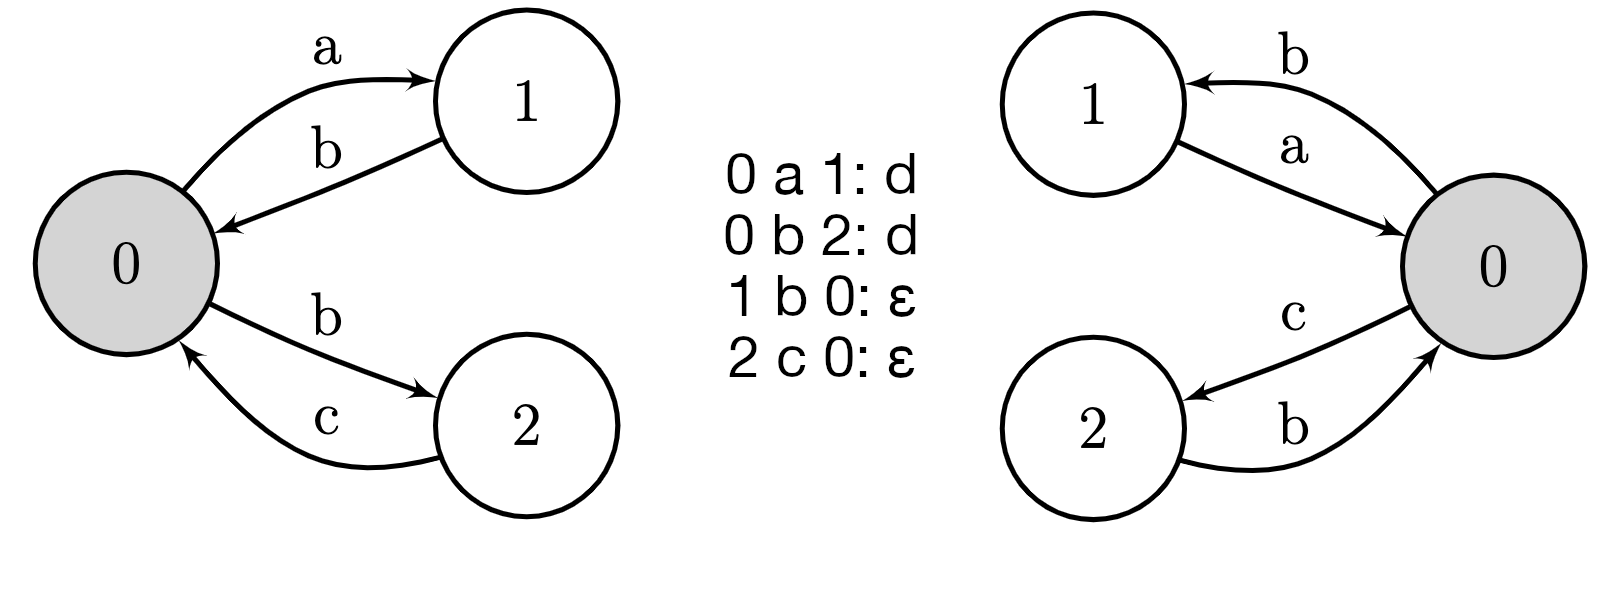
\includegraphics[
		width=12cm,
		height=6cm,
		keepaspectratio,
	  ]{img/bm.png}
	\caption{Бимашина представяща \( \{ \langle ab, d \rangle, \langle bc, d \rangle \}^* \)}
	\label{fig:Bm}
\end{figure}

\begin{example}{\emph{(Бимашина и изпълнение)}}
	Нека разлгледаме бимашината на Фигура \ref{fig:Bm}. Задаваме входна дума \emph{bcabbc}, което води до следното изпълнение на левия и десния автомат съответно.

	\[ \pi_L = 0 \to^{b} 2 \to^{c} 0 \to^{a} 1 \to^b 0 \to^{b} 2 \to^{c} 0 \]
	\[ \pi_R = 0 \leftarrow^{b} 2 \leftarrow^{c} 0 \leftarrow^{a} 1 \leftarrow^{b} 0 \leftarrow^{b} 2 \leftarrow^{c} 0 \]

	Изходната функция на бимашината \(\mathcal{O_B} \) прилагаме както следва:
	\[
		\psi(0,b,2) \cdot \psi(2,c,0) \cdot \psi(0,a,1) \cdot \psi(1,b,0) \cdot \psi(0,b,2) \cdot \psi(2,c,0) =
	d \cdot \epsilon \cdot d \cdot \epsilon \cdot d \cdot \epsilon = ddd
	\]

\end{example}

\begin{definition}
	Бимашина \( \mathcal{B} = \langle \mathcal{A}_L, \mathcal{A}_R, \psi \rangle \) наричаме \emph{тотална}, ако функциите на прехода \( \delta_L: Q_L \times \Sigma \to Q_L \) и \( \delta_R: Q_R \times \Sigma \to Q_R \) на левия и десния автомат съответно, както и функцията на изхода \( \psi: (Q_L \times \Sigma \times Q_R) \to \Sigma^* \) са \emph{тотални}.
\end{definition}

\begin{theorem}
	Класическите бимашини са еквивалентни по изразителност на регулярните функции. \cite{Schutzenberger:61} \cite{Mihov:2018-2}
\end{theorem}

\pagebreak
\section{Лексически анализ чрез регулярни релации}

\subsection{Правила за заместване}

На двоичните стрингови релации можем да гледаме като на множество от преводи. На пример за двойката думи \( \langle u, v \rangle \), където \(u,v \in \Sigma^*\), казваме, че думата \( u \) се превежда като \( v \).

\begin{definition}
	\emph{Правило за заместване} представяме във вида
	\[ E \to \beta \]
	където \( E \) е регулярен израз, а \( \beta \in \Sigma^* \) е дума.
	\emph{Приложение на правилото върху текст} \( t \in \Sigma^* \) представлява заместването на поднизовете на \( t \), които са в езика \( L(E) \) с думата \( \beta \).
\end{definition}

\begin{figure}[!htb]
	\centering
	\begin{tikzpicture}
		\node[font=\Large] {
			\( a_1a_2 \dots a_i \dots a_{i+k} \dots a_{j} \dots a_{j+l} \dots a_n \)
		};
		\draw [decorate,decoration={brace,amplitude=5pt,raise=0pt},yshift=0pt]
		(-2.75,0.4) -- (-0.25,0.4) node [black,midway,xshift=0cm,yshift=0.5cm] {\footnotesize $ \in L(E) $};
		\draw [decorate,decoration={brace,amplitude=5pt,mirror,raise=0pt},yshift=0pt]
		(-2.75,-0.3) -- (-0.25,-0.3) node [black,midway,xshift=0cm,yshift=-0.5cm] {\footnotesize $ \beta $};
		\draw [decorate,decoration={brace,amplitude=5pt,raise=0pt},yshift=0pt]
		(0.8,0.4) -- (3.15,0.4) node [black,midway,xshift=0cm,yshift=0.5cm] {\footnotesize $ \in L(E) $};
		\draw [decorate,decoration={brace,amplitude=5pt,mirror,raise=0pt},yshift=0pt]
		(0.8,-0.3) -- (3.15,-0.3) node [black,midway,xshift=0cm,yshift=-0.5cm] {\footnotesize $ \beta $};
	\end{tikzpicture}
	\caption{Приложение на правило на заместване}
\end{figure}

\noindent \emph{Правила за заместване} можем да представим като \emph{регулярни стрингови релации}, използвайки единствено алгебрата на регулярните езици и релации. Те се реализират програмно чрез крайни преобразуватели \cite{Kaplan&Kay:94}.

\begin{definition}
	Нека разгледаме текст \( t \in \Sigma^* \). \emph{Срещане} на \emph{v} наричаме тройка \( \langle u,v,w \rangle \), където \( t = uvw \). Също така \( u \) и \( w \) наричаме съответно \emph{префикс} и \emph{суфикс} на срещането, докато \( v \) наричаме \emph{инфикс}.
\end{definition}

\begin{example}
	Нека разгледаме правилото \verb/ab|bc/ \( \to d \). След приложението му над текста \emph{abb}, ще получим \emph{db}, като \( \langle \epsilon, ab, b \rangle \) е единственото срещане. Приложението на правилото над \emph{abbacbca} ще доведе до \emph{dbacda} две срещания \( \langle \epsilon, ab, bacbca \rangle \) и \( \langle abbac, bc, a \rangle \).
\end{example}

\subsection{Разрешаване на многозначности}

При прилагане на правило за заместване могат да възникнат многозначности в случаите, в които две срещания имат застъпващи се инфикси.

\begin{definition}
	Две срещания \( \langle u_1,v_1,w_1 \rangle \) и \( \langle u_2,v_2,w_2 \rangle \) за даден текст \( t \) \emph{се застъпват}, ако \( u_1 < u_2 < u_1v_1 \). Израза \( u_1 < u_2 \) четем като \( u_1 \) е \emph{префикс} на \( u_2 \).
\end{definition}

\begin{figure}[!htb]
	\centering
	\begin{tikzpicture}
	\draw (0,0) rectangle (3,1); % u_1
	\draw (0,0) rectangle (5,1); % u_2
	\draw[pattern=horizontal lines] (3,0) rectangle (7,1); % v_1
	\draw[pattern=vertical lines] (5,0) rectangle (8,1); % v_2
	\draw (7,0) rectangle (11,1); % w_1
	\draw (8,0) rectangle (11,1); % w_2
	\draw [decorate,decoration={brace,amplitude=10pt,raise=3pt},yshift=0pt]
		(0,1) -- (3,1) node [black,midway,xshift=0cm,yshift=0.75cm] {\footnotesize $u_1$};
	\draw [decorate,decoration={brace,amplitude=10pt,mirror,raise=3pt},yshift=0pt] 
		(0,0) -- (5,0) node [black,midway,xshift=0cm,yshift=-0.75cm] {\footnotesize $u_2$};
	\draw [decorate,decoration={brace,amplitude=10pt,raise=3pt},yshift=0pt]
		(3,1) -- (7,1) node [black,midway,xshift=0cm,yshift=0.75cm] {\footnotesize $v_1$};
	\draw [decorate,decoration={brace,amplitude=10pt,mirror,raise=3pt},yshift=0pt]
		(5,0) -- (8,0) node [black,midway,xshift=0cm,yshift=-0.75cm] {\footnotesize $v_2$};
	\draw [decorate,decoration={brace,amplitude=10pt,raise=3pt},yshift=0pt]
		(7,1) -- (11,1) node [black,midway,xshift=0cm,yshift=0.75cm] {\footnotesize $w_1$};
	\draw [decorate,decoration={brace,amplitude=10pt,mirror,raise=3pt},yshift=0pt]
		(8,0) -- (11,0) node [black,midway,xshift=0cm,yshift=-0.75cm] {\footnotesize $w_2$};
	\end{tikzpicture}
	\caption{Многозначност - срещания, чиито инфикси се застъпват}
\end{figure}

\begin{example}
	Нека разгледаме правилото \verb/ab|bc/ \( \to d \) приложено над текста \( t = aabcb \). Получаваме срещанията \( \langle a, ab, cb \rangle \) и \( \langle aa, bc, b \rangle \), които очвевидно се застъпват и съответно стигаме до две различни валидни замествания \emph{adcb} и \emph{aadb}.
\end{example}

\begin{figure}[!htb]
	\centering
	\begin{tikzpicture}
	\draw (0,0) rectangle (3,1); % u_1
	\draw (0,0) rectangle (3,1); % u_2
	\draw[pattern=horizontal lines] (3,0) rectangle (8,1); % v_1
	\draw[pattern=vertical lines] (3,0) rectangle (6,1); % v_2
	\draw (8,0) rectangle (11,1); % w_1
	\draw (6,0) rectangle (11,1); % w_2
	\draw [decorate,decoration={brace,amplitude=10pt,raise=3pt},yshift=0pt]
		(0,1) -- (3,1) node [black,midway,xshift=0cm,yshift=0.75cm] {\footnotesize $u_1$};
	\draw [decorate,decoration={brace,amplitude=10pt,mirror,raise=3pt},yshift=0pt] 
		(0,0) -- (3,0) node [black,midway,xshift=0cm,yshift=-0.75cm] {\footnotesize $u_2$};
	\draw [decorate,decoration={brace,amplitude=10pt,raise=3pt},yshift=0pt]
		(3,1) -- (8,1) node [black,midway,xshift=0cm,yshift=0.75cm] {\footnotesize $v_1$};
	\draw [decorate,decoration={brace,amplitude=10pt,mirror,raise=3pt},yshift=0pt]
		(3,0) -- (6,0) node [black,midway,xshift=0cm,yshift=-0.75cm] {\footnotesize $v_2$};
	\draw [decorate,decoration={brace,amplitude=10pt,raise=3pt},yshift=0pt]
		(8,1) -- (11,1) node [black,midway,xshift=0cm,yshift=0.75cm] {\footnotesize $w_1$};
	\draw [decorate,decoration={brace,amplitude=10pt,mirror,raise=3pt},yshift=0pt]
		(6,0) -- (11,0) node [black,midway,xshift=0cm,yshift=-0.75cm] {\footnotesize $w_2$};
	\end{tikzpicture}
	\caption{Застъпващи се срещания с еднакво начало}
\end{figure}

\begin{example}
	Друг вид многозначност може да получим, когато инфиксите на две срещания имат еднакво начало. Например, ако приложим правилото \( \verb/a+/ \to d \) над тескт \( t = aa \), може получим превода \emph{dd}, на който отговарят срещанията \( \langle \epsilon, a, a \rangle \) и \( \langle a, a, \epsilon \rangle \), и \emph{d} със срещане \( \langle \epsilon, aa, \epsilon \rangle \).
\end{example}

Разрешаването на такъв тип многозначности, ще постигнем като реализираме стратегията \emph{най-ляво-най-дълго} срещане. Измежду две застъпващи се срещания, ще избираме това, чийто инфикс е в най-лява позиция. Ако инфиксите започват от една и съща позиция, ще избираме срещането с най-дълъг инфикс.

\begin{definition}
	Нека \(A = \{ \langle u_1, v_1, w_1 \rangle, \dots , \langle u_k, v_k, w_k \rangle \}\) е множество от \emph{незастъпващи се} срещания на текст \(t \in \Sigma^*\) и \(k = |A|\), където \( u_jv_j < u_{j+1} \) за \( 1 \le i < j < k \). \emph{Каноничното представяне} на \(t\) за \(A\) е редицата от \(2k+1\) думи \( \langle u_1, v_1, x_2, v_2, \dots , x_k, v_k, w_k \rangle \), където \( x_i = [u_{i-1}v_{i-1}]^{-1}u_i \) за \( 2 \le i \le k \). Текстът \(t\) получаваме като конкатенираме на елементите в редицата \(t = u_1v_1x_2v_2 \dots x_kv_kw_k \). Очевидно е, че от тази редица също можем да изведем множеството от незастъпващи се срещания \(A\).
\end{definition}

\begin{example}
	Нека \( t = aabcbcab, A = \{ \langle a, ab, cbcab \rangle, \langle aabc, bc, ab \rangle, \langle aabcbc, ab, \epsilon \rangle \} \). \emph{Каноничното представяне} на \(t\) за \(A\) е редицата
	\[ \langle u_1, v_1, x_2, v_2, x_3, v_3, w_3 \rangle = \langle a, ab, c, bc, \epsilon, ab, \epsilon \rangle \]
\end{example}

\begin{definition}\label{def:LmlOps}
	Въвеждаме следните оператори над множества от срещания:
\[ AFTER(A, B) = \{ \langle u, v, w \rangle \in A \mid \forall \langle u', v', w' \rangle \in B : u'v' \leq u \land u' < u  \} \] 

\( AFTER \) избира измежду всички срещания в множеството \(A\) тези, в които инфиксът \(v\) започва след всички инфикси в множеството \(B\).

\[ LEFT(A) = \{ \langle u, v, w \rangle \in A \mid \forall \langle u', v', w' \rangle \in A : u \leq u' \} \]

\( LEFT \) избира измежду всички срещания в \(A\), тези с чийто инфикс се намира възможно най в ляво. Може да имаме повече от едно такова срещане.

\[ LONG(A) = \{ \langle u, v, w \rangle \in A \mid \forall \langle u', v', w' \rangle \in A : u \neq u' \lor v' \leq v \} \]

Измежду срещанията, чиито инфикси започват от една и съща позиция, \( LONG \) избира тези, които имат най-дълъг инфикс.
\end{definition}

\begin{definition}
	Използвайки операторите от дефиниция \ref{def:LmlOps}, въвеждаме функцията \( LML(A) \) (\emph{leftmost-longest}). По зададено множество от срещания \(A\), \( LML(A) \) извежда множество от незастъпващи се срещания, като избира най-левите, най-дълги измежду тях.
	\[ LML(A) := \bigcup\limits_{i=0}^{\infty} V_{i} \]
	където множествата \( V_i \) строим индуктивно
	\[ V_0 := \emptyset \]
	\[ V_{i+1} := V_i \cup LONG(LEFT(AFTER(A, V_i))) \]

	\noindent \( LML(A) \) е крайно множество, защото \( A \) е крайно, т.е. след даден момент редицата ще престане да нараства.
\end{definition}

\begin{proposition}
	Нека \( t \in \Sigma^* \) е текст и \(A\) е множество от срещания спрямо \(t\). \( LML(A) \) съдържа само незастъпващи се срещания.

	\begin{proof}
		Нека \( LML(A) \) съдържа застъпващите се срещания \( \langle u_1, v_1, w_1 \rangle \) и \( \langle u_2, v_2, w_2 \rangle \) т.е. \( u_1 < u_2 < u_1v_1 \). Също така \( \langle u_1, v_1, w_1 \rangle \) и \( \langle u_2, v_2, w_2 \rangle \) са били добавени съответно за пръв път в \( V_{i_1} \text{ и } V_{i_2} \).
		\begin{enumerate}
			\item Нека \( i_1 \geq i_2 \), тогава
			\[ \langle u_2, v_2, w_2 \rangle \in V_{i_2} = V_{i_2-1} \cup LONG(LEFT(AFTER(A, V_{i_2-1}))) \]
			\noindent След като \( \langle u_2, v_2, w_2 \rangle \notin V_{i_2-1} \), то 
			\[ \langle u_2, v_2, w_2 \rangle \in LEFT(AFTER(A, V_{i_2-1})) \]
			От допускането, че \( i_1 \geq i_2 \) следва, че 
			\[ \langle u_1, v_1, w_1 \rangle \in AFTER(A,V_{i_2-1}) \]
			Двете срещания са във входното множество на функцията \emph{LEFT}, но тъй като \( u_1 < u_2 < u_1v_1 \), по дефиницията на \emph{LEFT}, \( \langle u_2, v_2, w_2 \rangle \) не може да се съдържа в \( LEFT(AFTER(A, V_{i_2-1})) \), следователно стигаме до противоречие.
			\item Нека \( i_1 < i_2 \), тогава \( \langle u_2, v_2, w_2 \rangle \notin V_i \) за \( i \leq i_1 \). При \( i > i_1 \), \( \langle u_1, v_1, w_1 \rangle \in V_i \), значи \( \langle u_2, v_2, w_2 \rangle \in AFTER(A, V_i) \), което не е възможно спрямо дефиницията на \( AFTER \) (избира срещанията в \(A\), чиито инфикси започват след края на инфиксите на тези в \(V_i\)) следователно \( \langle u_2, v_2, w_2 \rangle \notin V_{i+1} \). Това противоречи с факта, че \( \langle u_2, v_2, w_2 \rangle \in V_{i_2} \) и \(i_1 < i_2 \), от където стигаме до извода, че \( LML(A) \) не съдържа застъпващи се срещания.
		\end{enumerate}
	\end{proof}
\end{proposition}

\begin{definition}
	\label{def:RlmlT}
	Нека \( T \subseteq \Sigma^* \times \Sigma^* \) е регулярна релация и \( t \in \Sigma^* \) е текст. С \( A_{dom(T)} \) бележим множеството на всички срещания от вида \( \langle u,v,w \rangle \) спрямо \(t\), чиито инфикси \(v\) са в \(dom(T)\). Нека \( \langle u_1, v_1, x_2, v_2, \dots, x_k, v_k, w_k \rangle \) е каноничното представяне на \(t\) за множеството \( LML(A_{dom(T)}) \). Тогава \(t'\) е \emph{заместването} на \(t\) с \(T\) под стратегията най-ляво-най-дълго срещане, ако: 
	\[t' = u_1 v_1' x_2 v_2' \dots x_k v_k' w_k\] 
	и \( \langle v, v' \rangle \in T \) за \( 1 \leq i \leq k \). С \( R^{LML}(T) \) бележим \emph{релацията на заместване под стратегията най-ляво-най-дълго срещане} за \(T\). Тя съдържа всички двойки \( \langle t, t' \rangle \in \Sigma^* \times \Sigma^* \), така че \( t' \) е заместване на \( t \) с \(T\) под стратегията най-ляво-най-дълго срещане.
\end{definition}

\begin{corollary}
	Нека \( T: \Sigma^+ \to \Sigma^* \) е функция, тогава релацията на заместване \( R^{LML}(T) \) е функционална. Това следва от факта, че думите \(u_1, x_i, w_k \) за \( 2 \le i \le k \) от каноничното представяне се превеждат с идентитет, а на всяка дума \( v_j \), където \( 1 \le j \le k \) съответства точно една дума \( v_j' \), така че \( T(v_j) = v_j' \).
\end{corollary}

\begin{example}
	Нека разгледаме правилото \verb/ab|bc/ \( \to d \), съответстващо на релацията \(T = \{ \langle ab,d \rangle, \langle bc, d \rangle \} \) и го приложим текста \( t = aabcbab \). Получаваме срещанията \( \langle a, ab, cbab \rangle \), \( \langle aa, bc, bab \rangle \) и \( \langle aabcb, ab, \epsilon \rangle \). Очевидно първите два се застъпват, но стратегията най-ляво-най-дълго срещане определя първият и третият за валидни. Каноничното представяне на \(t \) e \( \langle a, ab, cb, ab, \epsilon  \rangle \) и резултатът от заместането е \( R^{LML}(T)(aabcbab) = adcbd \).
\end{example}

\subsection{Релация за лексически анализ}
\label{sec:LexARegRel}
Регулярните релации намират своето приложение в множество домейни, като лексическият анализ е един от тях. Идеята е да сведем процеса до заместване на думи в текст, като по лексическата граматика построим релация на заместване под стратегията \emph{най-ляво-най-дълго срещане}. Тази релация реализираме програмно чрез краен преобразувател, който маркира всяка разпозната лексема. В последствие по него строим еквивалентна бимашина следвайки \cite{GerdjikovEtAl:2017}, \cite{Mihov:2018-2}.

Ще представим формално конструкция на релация на заместване под стратегията най-ляво-най-дълго срещане, по метода на Карттунен (1996) \cite{Karttunen:96}. Целта ни е по зададена регулярна релация \(T\), да построим релация на заместваме по стратегията най-ляво-най-дълго срещане, съответстваща на \( R^{LML}(T) \) (Дефиниция \ref{def:RlmlT}). В последствие ще използваме тази конструкция, за да построим релация за лексически анализ.

Като начало дефинираме множеството на маркерите, които ще използваме по време на междинните стъпки за извършване на заместването \( \Gamma = \{ \textasciicircum, <, > \} \). Това са произволни символи извън азбуката на еквивалентния преобразувател на \(T\), \( \Sigma \cap \Gamma = \emptyset \). Множеството на всички символи бележим със \( \Sigma_m = \Sigma \cup \Gamma \).

\begin{definition}
	Представяме следните оператори над регулярни езици:
	\[ not(L) = \{ w \mid w \in \Sigma_m^* \land w \notin L \} \]
	\[ contain(L) = \{ w \mid w_1w_2w_3 = w: w_1, w_3 \in \Sigma_m^* \land w_2 \in L \} \]
	С \( not(L) \) получаваме допълнението на езика \(L\), \( contain(L) \) връща езика, който се състои от всички думи, които съдържат инфикс в \(L\). Строим функциите по следния начин:
	\[ not(L) := \Sigma_m^* \setminus L \]
	\[ contain(L) := \Sigma_m^* \cdot L \cdot \Sigma_m^* \]
\end{definition}

\begin{corollary}
	\emph{not(L)} и \emph{contain(L)} са регулярни езици, тъй като са построени чрез операциите \emph{звезда, конкатенация} и \emph{разлика}, а регулярните езици са затворени относно тези операции.
\end{corollary}

\begin{definition}
	Представяме групата от оператори \(intro\), въведени първоначално от Каплан и Кей (1994) \cite{Kaplan&Kay:94}:
	\[ intro(S) := (Id(\Sigma_m \setminus S) \cup (\{\epsilon\} \times S))^* \]
	\[ introx(S) := (intro(S) \cdot Id(\Sigma_m \setminus S)) \cup \{\langle \epsilon, \epsilon \rangle \} \]
	\[ xintro(S) := (Id(\Sigma_m \setminus S) \cdot intro(S)) \cup \{\langle \epsilon, \epsilon \rangle \} \]
	\emph{intro(S)} създава релация, която добавя произволно символи от \(S\) в думи, които не съдържат символи от \(S\), \emph{introx(S)} и \emph{xintro(S)} са аналогични, като символите от \(S\) не могат да се намират съответно в края и началото на изходната дума.
\end{definition}

\begin{example}
	Имаме регулярният език \( \{a,b\} \), в който \emph{въвеждаме} символите от \(S := \{ x \}\). Тогава релацията \(intro(S)\) ще съдържа двойките \( \langle b, xb \rangle, \langle ab, axbx \rangle, \langle abba, axxbbax \rangle \dots \)
\end{example}

\begin{corollary}
	Регулярните езици са затворени относно разлика. Прилагайки операциите за \emph{идентитет и произведение} над регулярни езици, получаваме регулярни релации. Регулярните релации са заторени относно \emph{обединение, конкатенация и звезда}, така че релациите, които \emph{intro, introx и xintro} строят са също регулярни.
\end{corollary}

\begin{definition}
	Преставяме групата от \emph{ignore} оператори както следва \cite{Kaplan&Kay:94}:
	\[ ignore(L,S) := range(Id(L) \circ intro(S)) \]
	\[ ignorex(L,S) := range(Id(L) \circ introx(S)) \]
	\[ xignore(L,S) := range(Id(L) \circ xintro(S)) \]
	По даден регулярен език \(L\) и множество от символи \(S\), \emph{ignore(L,S)} връща регулярен език, който се състои от думите в \(L\), със свободно включени символи от \(S\). \emph{ignorex(L,S), xignore(L,S)} са аналогични като не включват символи от \(S\) съответно в края и в началото на думите.	
\end{definition}

\begin{example}
	Нека разгледаме регулярният език \(L(E)\), представен от израза \( E = \verb/(a|b)+/ \). Този език се състои от всички думи с дължина поне един символ, които съдържат произволен брой \emph{'a'} и \emph{'b'}. \( L(E) = \{a, b, ba, ab, ababb \dots \} \), \( ignore(L(E), \{x\}) \) ще съдържа думите \emph{ab, xa, xab, xabxxb, bbb, bxabx \dots }
\end{example}

\begin{corollary}
	Реуглярните релации са затворени относно композиция и кодомейна на регулярна релация е регулярен език. Следователно операторите \emph{ignore, ignorex, xignore} строят регулярни езици.
\end{corollary}

\begin{definition}\label{def:defIfPThenS}
	Въвеждаме следните функции, над регулярни езици \cite{Kaplan&Kay:94}:
	\[ ifPthenS(P,S) = \{ w \mid \forall w_1w_2 = w: \text{ ако } w_1 \in P \text{ то } w_2 \in S \} \]
	\[ ifSthenP(P,S) = \{ w \mid \forall w_1w_2 = w: \text{ ако } w_2 \in S \text{ то } w_1 \in P \} \]
	\emph{ifPthenS(P,S)} дефинира езика, на чиито думи, ако префиксите им са в езика \(P\) то суфиксите са в \(S\). Аналогично \emph{ifSthenP(P,S)} представя думите, за които ако имат суфикс в \(S\), то съответния префикс е в \(P\). Реализираме тези функции както следва:
	\[ ifPthenS(P,S) := not(P \cdot not(S)) \]
	\[ ifSthenP(P,S) := not(not(P) \cdot S) \]	
\end{definition}

\begin{definition}
	Комбинираме операторите от дефиниция \ref{def:defIfPThenS}, за да представим:
	\[ PiffS(P,S) = \{ w \mid \forall w = w_1w_2: w_1 \in P \leftrightarrow w_2 \in S \} \]
	\[ LiffR(L,R) = \{ w \mid \forall w = w_1w_2w_3: \forall w_2'w_2'' = w_2: w_2' \in L \leftrightarrow w_2'' \in R \} \]
	\emph{PiffS(P,S)} строи автомат, разпознаващ думите, чиито префикси са в \(P\) тогава и само тогава, когато суфиксите им са в \(S\). \emph{LiffR(L,R)} съдържа думите \( w = w_1w_2w_3 \), така че префиксите на \(w_2\) са в \(L\) и суфиксите на \(w_2\) са в \(R\). Реализираме тези функции както следва:
	\[ PiffS(P,S) := ifPthenS(P,S) \cap ifSthenP(P,S) \]
	\[ LiffR(L,R) := PiffS((\Sigma_m^* \cdot L), (R \cdot \Sigma_m^*)) \]	
\end{definition}

\begin{corollary}
	\emph{ifPthenS, ifSthenP, PiffS, LiffR} са резултат от приложението на операциите над регулярни езици - \emph{допълнение, конкатенация, сечение и звезда}. От свойствата на затваряне следва, че езиците, построени от тези оператори са също регулярни.
\end{corollary}

\begin{definition}\label{def:Robl}
	Нека \(T \subseteq \Sigma^* \times \Sigma^* \) е регулярна релация. \emph{Релацията на задължително (obligatory) заместване} \(R^{obl}(T)\) дефинираме както следва:
	\[ R^{obl}(T) := N(T) \cdot (T \cdot N(T))^* \]
	\[ N(T) := Id(\Sigma_m^* \setminus (\Sigma_m^* \cdot dom(T) \cdot \Sigma_m^*)) \cup \{ \langle \epsilon, \epsilon \rangle \} \]
	\(N(T)\) е идентитетът на множеството от всички думи, които не съдържат инфикси в \(dom(T)\) обединен с двойката \(\langle \epsilon, \epsilon \rangle\), заместваща празната дума с празната дума.
	Идеята е следната - поддумите от входа, които са в \(dom(T)\) се превеждат спрямо \(T\), докато тези, които не са в домейна ѝ се превеждат чрез идентитет, т.е. входът там остава непроменен.
\end{definition}

\begin{example}
	Нека разгледаме следния пример: \(T = \{ \langle ab, d \rangle, \langle bc, d \rangle \} \) и имаме \(R^{obl}(T) \). Входният текст \( t_1 = babacbca \) се декомпозира като:
	\[ t_1 = b \cdot ab \cdot ac \cdot bc \cdot a \]
	Поддумите \(\{b, ac, a\} \subseteq dom(N(T))\), докато \(\{ab, bc\} \subseteq dom(T)\). Съответно след заместването получаваме
	\[ t_1' = b \cdot d \cdot ac \cdot d \cdot a \]
	За входният текст \( t_2 = abcc \) обаче имаме две валидни композиции:
	\[ t_2 = ab \cdot cc = a \cdot bc \cdot c \]
	Това ще доведе до два възможни превода, т.е. \( \langle abcc, dcc \rangle \in R^{obl}(T) \) и \( \langle abcc, adc \rangle \in R^{obl}(T) \).
\end{example}

\begin{corollary}
	От свойствата на затваряне над регулярни езици и релации следва, че \(R^{obl}(T)\) също е регулярна.
\end{corollary}

Вече сме готови да дефинираме основните релации по \cite{Karttunen:96}. Започваме с тази за първоначално срещане.

\begin{definition}\label{def:Rinit} \emph{Релация на първоначално срещане} представяме както следва:
	\[ R^{init}(T) := intro(\{ \text{\textasciicircum} \}) \circ Id \Big(LiffR \big(\{ \text{\textasciicircum} \}, xignore(dom(T), \{ \text{\textasciicircum} \}) \big) \Big) \]

	\( R^{init}(T) \) поставя маркерa \textasciicircum \hspace*{0cm} в началото на всяко срещане на поддума (инфикс) от входния текст, която е в домейна на \(T\). Тази стъпка идентифицира началото на инфиксите на всички срещания на заместване в текста независимо от това дали се застъпват, или са с възможно най-дълги инфикси. Тя отговаря на определянето на входното множество от срещания \(A\) (Дефиниция \ref{def:LmlOps}).
\end{definition}

\begin{definition}\label{def:Rleft} \emph{Релация на най-ляво срещане} представяме както следва:
	\begin{equation}
		\begin{split}
			R^{left}(T) :=
			\bigg( \bigg( \Big( Id(\Sigma^*) \cdot \{ \langle \text{\textasciicircum}, < \rangle \} \cdot Id \big(ignorex(dom(T), \{ \langle \epsilon, > \rangle \})\big) \Big)^* \bigg) \cdot Id(\Sigma^*) \bigg) \\ 
			\circ R^{obl} (\{ \langle \text{\textasciicircum}, \epsilon \rangle \}) 
		\end{split}
	\end{equation}

	\(R^{left}(T)\) получава текст с маркерите (\textasciicircum) от първатата стъпка (\(R^{init}(T)\)) и поставя в началото и края на всяко срещане маркерите < и >, като  \textasciicircum \hspace*{0cm} се замества с <. Между маркерите за начало и край, не може да съществуват други маркери. Това може да доведе до повече от един изходен текст, като единият от тях маркира коректно срещанията спрямо стратегията \emph{най-ляво-най-дълго срещане}. Тази стъпка отговаря на композицията на операторите \(AFTER \circ LEFT\) (Дефиниция \ref{def:LmlOps}) и осигурява, че измежду срещанията със застъпващи се инфикси, ще останат само тези, чийто инфикс се намира най-ляво спрямо входния текст. \( R_{obl} (\{ \langle \text{\textasciicircum}, \epsilon \rangle \}) \) изтрива останалите маркери, поставени в предходната стъпка, които са останали в сегментите между < и >.
\end{definition}

\begin{definition}\label{def:Rlong} \emph{Релация на най-дълго срещане} представяме както следва:
	\[ R^{long}(T) := Id \bigg( not \Big(contain \big(\{<\} \cdot \big(ignorex(dom(T), \{<, >\}) \cap contain(\{>\})\big) \big) \Big) \bigg) \]
	Релацията получава изхода от втората съпка (\(R^{left}(T)\)) и измежду маркираните текстове съдържащи срещания с еднакво начало, извежда такъв, в който инфиксите са най-дълги. Тази стъпка отговаря на оператора \(LONG\).
\end{definition}

\begin{definition}\label{def:Rreplace} \emph{Релация на заместване} представяме както следва:
	\[ R^{replace}(T) := R^{obl}(\{ \langle <, \epsilon \rangle \} \cdot T \cdot \{ \langle >, \epsilon \rangle \}) \]
	В тази стъпка получаваме изходния текст на \(R^{long}\), в който поддумите в домейна на преобразувателя са маркирани с < и > под стратегията най-ляво-най-дълго срещане. Този преобразувател извършва заместването на тези поддуми чрез входния преобразувател и премахва маркерите.
\end{definition}

\begin{example}
	Имаме релациите \( R_1, R_2 \), съответстващи на правилата на заместване \verb/ab+/ \( \to x \) и \verb/bc/ \( \to y \). \(R_1\) замества думите, започващи с \emph{a}, последвано от едно, или повече \emph{b} с \emph{x}. \(R_2\) замества думата \emph{bc} с \emph{y}. Релацията \(T\) получаваме като ги обединим: \( T := R_1 \cup R_2 \). Имаме входния текст \emph{t = abcabbdbc} и маркерите \textasciicircum, < и >. Симулираме процеса на заместване както следва:
	\begin{enumerate}
		\item Маркираме началото на всички инфикси в думата: \\ \( R^{init}(T)(abcabbdbc) = \) \emph{\textasciicircum a\textasciicircum bc\textasciicircum abbd\textasciicircum bc}
		\item Идентифицираме най-левите незастъпващи се срещания, което води до следните възможни декомпозиции: \\ 
		\( \langle \textasciicircum a\textasciicircum bc\textasciicircum abbd\textasciicircum bc,\) \emph{<ab>c<ab>bd<bc>} \(\rangle \in R^{left}(T) \) \\
		\( \langle \textasciicircum a\textasciicircum bc\textasciicircum abbd\textasciicircum bc,\) \emph{<ab>c<abb>d<bc>} \(\rangle \in R^{left}(T) \)
		\item Релацията за най-дълго срещане филтрира думите, чиито маркери не следват съответното изискване: \\
		<ab>c<ab>bd<bc> \( \notin dom(R^{long}(T)) \) \\
		\( R^{long}(T)(\)<ab>c<abb>d<bc>\() = \) <ab>c<abb>d<bc>
		\item Заместваме поддумите, оградени с маркери, спрямо релацията \(T\), трием маркерите и получаваме : \\
		\( R^{replace}(T)(\)<ab>c<abb>d<bc>\() = xcxdy \)
	\end{enumerate}
\end{example}

\begin{definition} \emph{Релация на заместване под стратегията "най-ляво-най-дълго срещане"} получаваме като композираме релациите дефинирани в \ref{def:Rinit}, \ref{def:Rleft}, \ref{def:Rlong}, \ref{def:Rreplace} , които строим независимо една от друга.

\[ R(T) = R^{init}(T) \circ R^{left}(T) \circ R^{long}(T) \circ R^{replace}(T) \]
\end{definition}

\begin{corollary}
	Релациите \( R^{init}(T), R^{left}(T), R^{long}(T) \) и \( R^{replace}(T) \) са регулярни, тъй като са построени след приложението на операции относно, които регулярните езици и релации са затоврени. От свойството, че регулярните релации са затворени относно композиция следва, че \( R(T)\) е също регулярна.
\end{corollary}

\begin{definition} \label{def:Rlex}
	Нека е дадена лексическата граматика
	\[ G := \langle E_1, E_2, \dots , E_n \rangle \]
	където \(n = |G|\) и \( E_i, i = 1, 2, \dots, n \) са регулярни изрази. Със символа \textasciicircum \hspace*{0cm} бележим началото на лексемите. Въвеждаме множество от символи \(X := \{ \sigma_1, \sigma_2, \dots, \sigma_n \}\), \(|X| = n\) като на с тях ще бележим края на лексемите. Всяко \(\sigma_i \in X\) отговаря на съответният регуларен израз \(E_i \in G\). Тези символи ни носят информация за типа, т.е. на кой от регулярните езици принадлежи разпознатата лексема.

	\noindent\emph{Релацията за лексически анализ} \(R^{lex}\) по граматиката \(G\) получаваме както следва:
	\[ T := \bigcup_{i=1}^{n} \{ \langle \epsilon, \hat{} \hspace*{0.1cm} \rangle \} 	\cdot Id(L(E_i)) \cdot \{ \langle \epsilon, \sigma_i \rangle \} \]
	\[ R^{lex} := R(T) \]

	За да гарантираме, че маркерите ще бъдат поставени по коректен начин, въвеждаме условието \( \Sigma \cap (X \cup \{ \hspace*{0.1cm} \hat{} \hspace*{0.1cm} \}) = \emptyset \), където \( \Sigma \) е азбуката на автомата \( \mathcal{A}_{L(E)} \), разпознаващ езика \(L(E)\), където
	\[ L(E) := \bigcup_{i=1}^{n} L(E_i) \]
\end{definition}

\begin{corollary}
	Ако \(T\) е функция, то \(R^{lex} \) е функция и по нея можем да построим еквивалентна бимашина. Това е изпълнено, ако не съществува дума \( w \in \Sigma^* \) и регулярни изрази \( E_i, E_j \in G \), така че \( w \in L(E_i)\text{ и } w \in L(E_j) \) и \( i \neq j \). Иначе казано, две правила в лексическата граматика не могат да разпознават една и съща дума.
\end{corollary}

\begin{figure}[!htb]
	\begin{center}
		\begin{tabular}{ |l|l| }
		\hline
		Token & Expression \\
		\hline
		\( E_1 \) & \verb/[0-9]+(\.[0-9]+)?/ \\
		\( E_2 \) & \verb/+|-|*|// \\
		\( E_3 \) & \verb/=/ \\
		\hline
		\end{tabular}
	\end{center}
	\caption{Лексическа граматика на аритметичен израз}
	\label{fig:ArGram}
\end{figure}

\begin{example}
	Нека разгледаме лексическата граматика на Фигура \ref{fig:ArGram}, по която сме построили релация за лексически анализ \(R^{lex}\). Избрали сме символите \emph{A,B,C}, които отговарят съответно на правила \(E_1, E_2 \text{ и } E_3 \). За входния текст \(t = 99.9+5= \) ще изведем следния резултат:
	\[ R^{lex}(\emph{99.9+5=}) = \verb/^99.9A^+B^5A^=C/ \]
	Изходният текст се състои от сегменти за всяка лексема, които са във вида \\ \emph{\textasciicircum<token-text><type-id> }.
\end{example}

% \subsection{Доказателство на конструкцията на релация на заместване по стратегията най-ляво-най-дълго срещане}

\subsection{Конструкция на бимашина}
\label{sec:BmConstruct}
Крайните преобразуватели са еквивалентни по изразителност на регулярните релации. С тях също така можем да представим и регулярните фунцкии при условие, че преобразувателят е недетерминиран. Детерминираните преобразуватели от своя страна не са достатъчно изразителни, така че да покрият изцяло класа на регулярните функции. За разлика от тях, бимашините могат да моделират регулярните стрингови функции \cite{Schutzenberger:61} като изцяло детерминистичен процес, с което задачите за заместване на думи в текст се решават за линейно време. В тази част ще представим формална конструкция на бимашина по зададен краен преобразувател, по метода представен в \cite{GerdjikovEtAl:2017} и \cite{Mihov:2018-2}.

Нека е даден функционален, тримован, краен преобразувател \( \mathcal{T} = \langle \Sigma \times \Sigma^*, Q, I, F, \Delta \rangle \), където \( \langle \epsilon, \epsilon \rangle \in L(\mathcal{T}) \). Целта ни е да построим бимашина \( \mathcal{B} = \langle \mathcal{A}_L, \mathcal{A}_R, \psi \rangle \), така че \( L(\mathcal{T}) = O_\mathcal{B} \).

Нека \( \mathcal{A_T} = \langle \Sigma, Q, I, F, \Delta_1 \rangle \) е подлежащият автомат на \( \mathcal{T} \) и \( \mathcal{A_T}^{rev} = \langle \Sigma, Q, F, I, \Delta_1^{rev} \rangle \) е огледалният на \( \mathcal{A_T} \). Десният автомат на бимашината, който симулираме по време на сканирането на входния текст от дясно на ляво, получаваме като детерминираме \( \mathcal{A_T}^{rev} \) и определим всички състояния за финални.
\[ \mathcal{A_R} = \mathcal{A_T}^{rev}_D = \langle \Sigma, Q_R, s_R, Q_R, \delta_R \rangle \]
където \( Q_R \subseteq 2^Q, s_R = F \) и функцията на прехода дефинираме както следва:
\[ \delta_R(R,a) = \{ q \in Q \mid \exists q' \in R, m \in \Sigma^* : \langle q, \langle a, m \rangle, q' \rangle \in \Delta \} \]
За да възстановим успешните пътища в \(\mathcal{T}\), ще съхраняваме допълнителна информация информация в състоянията на левия автомат. За целта дефинираме \emph{функцията на избор на състояние} \( \phi:Q_R \to Q \), която по дадено състояние \(P \in Q_R \) на десния автомат (което представлява множество от състояния в \(\mathcal{T}\)) избира едно от тези състояния \( \phi(P) = p \text{, където } p \in P \subseteq Q \). Дефинираме левия автомат на бимашината както следва:

\[ \mathcal{A_L} = \langle \Sigma, Q_L, s_L, Q_L, \delta_L \rangle \]

където множеството на състоянията \( Q_L \subseteq 2^Q \times 2^{Q_R \times Q} \) са двойки, съставени от множества от състояния на \(\mathcal{T}\) и функция за избор на състояние \(\phi\). Както при \(\mathcal{A_R}\), така и в \(\mathcal{A}_L\) всички състояния са финални. Дефинираме състоянията и функцията на прехода както следва:

\begin{itemize}
	\item \( s_L := \langle I, \phi_0 \rangle \), \( \phi_0(R) :=  
	\begin{cases} 
		\text{произволен елемент от } R \cap I & \text{ако } R \cap I \neq \emptyset \\
		\text{недефинирано} & \text{в прот. случай} \\
	\end{cases} \)
	\item За всяко \( \langle L, \phi \rangle \in Q_L \text{ и } a \in \Sigma \text{, } \delta_L(\langle L, \phi \rangle, a) := \langle L', \phi' \rangle \), където:
	\begin{itemize}
		\item \( L' := \{ q' \mid \exists q \in L, m \in \Sigma^* : \langle q, \langle a, m \rangle, q' \rangle \in \Delta \} \)
		\item \( \phi'(R') := 
		\begin{cases}
			\text{произволен елемент от } \\
			\{ q' \in R' \mid \exists m \in \Sigma^* : \langle q, \langle a, m \rangle, q' \rangle \in \Delta \} & \text{ако } q = \phi(\delta_R(R', a)) \text{ e деф.} \\
			\text{недефинирано} & \text{в прот. случай}
		\end{cases} \)
	\end{itemize}
\end{itemize}

От дефиницията на функцията на прехода \( \delta_R \) следва, че ако \( q = \phi(\delta_R(R', a)) \) е дефинирано, то множеството \( L' \neq \emptyset \) и \( \phi'(R') \) може да се дефинира по посочения начин.

Дефинираме \emph{функцията на изхода} \(\psi\) на бимашината, която по зададена двойка състояния \(\langle L, \phi \rangle\) и \(R'\) съответно на левия и десния автомат и буква \( a \in \Sigma \), нека \( \langle L', \phi' \rangle := \delta_L(\langle L, \phi \rangle, a) \) и \( R := \delta_R(R', a) \). Тогава

\[
	\psi(\langle L, \phi \rangle, a, R') := 
	\begin{cases}
		\text{произволен елемент от} \\
		\{ m \mid \langle \phi(R), \langle a, m \rangle, \phi'(R') \rangle \in \Delta \} & \text{ако } \phi(R) \text{ е деф.} \\
		\text{недефинирано} & \text{в прот. случай}
	\end{cases}
\]

Ако \( q = \phi(R) \) е дефинирано, тогава \( \{ q' \in R' \mid \exists m \in \Sigma^* : \langle q, \langle a, m \rangle, q' \rangle \in \Delta \} \neq \emptyset \). От дефиницията на \( \phi'(R') \) следва, че \( \{ m \mid \langle \phi(R), \langle a, m \rangle, \phi'(R') \rangle \in \Delta \} \neq \emptyset \) и \( \psi(\langle L, \phi \rangle, a, R') \) може да се дефинира по посочения начин. Доказателство за коректност на конструкцията е представено в оригиналната статия \cite{GerdjikovEtAl:2017}, както и в \cite{Mihov:2018-2}.

\begin{figure}[!htb]
	\centering
	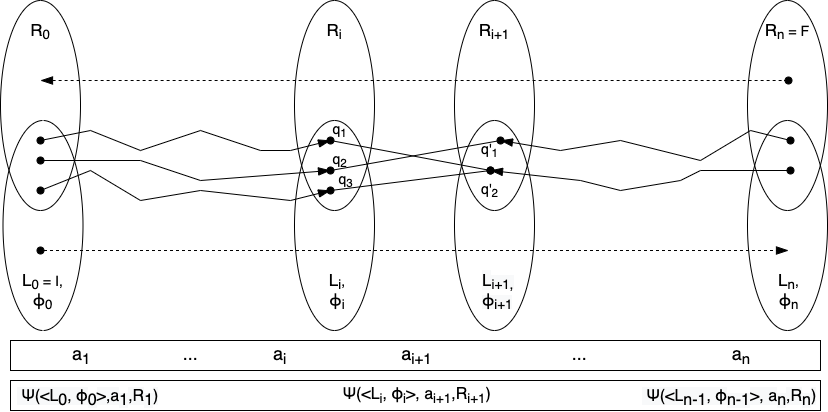
\includegraphics[
		width=15cm,
		keepaspectratio
	  ]{img/fst-bm.png}
	\caption{Симулация на преобразувател в контекста на еквивалентната му бимашина.}
	\label{fig:FstBm}
\end{figure}

Нека разгледаме Фигура \ref{fig:FstBm}. Дадена е входна дума \(w = a_1 ... a_n \in dom(L(\mathcal{T}))\) и \(\mathcal{T}\) се намира в множеството от начални състояния \( I = L_0 \). Когато \(\mathcal{T}\) се намира в състояния \(L_i, i = 1, \dots, n \) и прочете \(a_{i+1} \), той преминава в \( L_{i+1} \), следвайки всички преходи от \( L_i \) по символа \( a_{i+1} \). Аналогично се извършва обхождането в обратната посока, където \( F = R_n \) е множеството от начални състояния, \(R_0\) са финалните, и от състояня \( R_{i+1}\) на прочетен символ \(a_{i+1}\), преминаваме в \(R_i\) следвайки преходите само че в обратна посока. Тъй като \(L_i \text{ и } R_i\) се намират на успешни пътища съответно в левия и десния автомат на бимашината, то в състоянията \(\{q \mid q \in L_i \cap R_i \} \) се намират на успешен път в \(\mathcal{T}\) и след прочитането на символа \( a_{i+1}\), следвайки преходите от тези състояния, \(\mathcal{T}\) преминава в състоянията \(\{ q' \mid q' \in L_{i+1} \cap R_{i+1} \}\). След като \(\mathcal{T}\) е функционален, изходните думи 
\[
	\{ m \in \Sigma^* \mid \exists q \in L_i \cap R_i, \exists q' \in L_{i+1} \cap R_{i+1} : \langle q, \langle a_{i+1}, m \rangle, q' \rangle \in \Delta \}
\]
на преходите от \(L_i \cap R_i\) към \(L_{i+1} \cap R_{i+1}\) съвпадат.

\begin{figure}[!htb]
	\begin{center}
		\begin{tabular}{ |l|l| } 
		\hline
		Token & Expression \\
		\hline
		\( E_1 \) & \verb/а/ \\
		\( E_2 \) & \verb/a+b/ \\
		\hline
		\end{tabular}
	\end{center}	
	\caption{Лексическа граматика}
	\label{fig:Lexgr3}
\end{figure}

\begin{figure}[!htb]
	\centering
	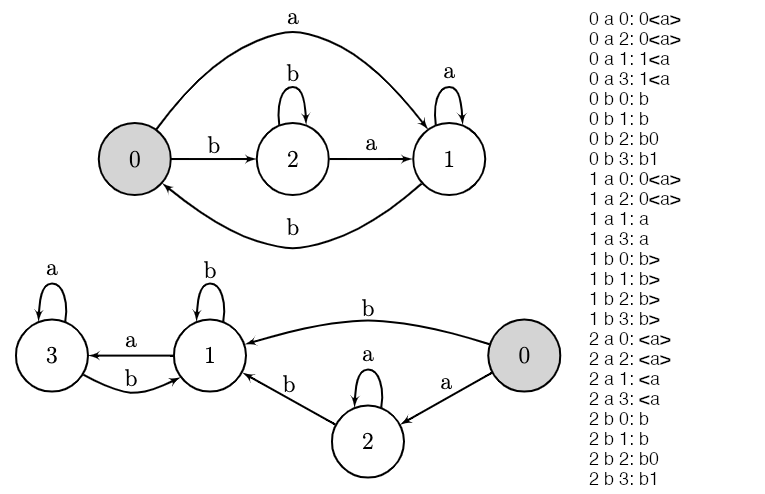
\includegraphics[
		width=14cm,
		keepaspectratio,
	  ]{img/bmlex.png}
	\caption{Бимашина за лексически анализ, построена по граматиката на Фигура \ref{fig:Lexgr3}}
	\label{fig:Bmlex}
\end{figure}

\begin{example}
	Нека разгледаме граматиката от Фигура \ref{fig:Lexgr3} и построената по нея бимашина на Фигура \ref{fig:Bmlex} спрямо представената конструкция в тази глава. Използваме \textasciicircum, за да маркираме началото и \(\{A,B\}\) за край на лексемите, като \emph{A} съотвества на \(E_1\), а \emph{B} на \(E_2\).
	Нека разгледаме входния текст \emph{aabaa}. Симулираме левия и десния автомат на бимашината и получаваме следните пътища:
	\[ \pi_L = 0 \to^{a} 1 \to^{a} 1 \to^{b} 0 \to^a 1 \to^a 1 \] 
	\[ \pi_R = 3 \leftarrow^{a} 3 \leftarrow^{a} 1 \leftarrow^{b} 2 \leftarrow^a 2 \leftarrow^a 0 \]
	Резултата получаваме като конкатенираме резултатите от функцията на изхода за всяка тройка, състояща се от ляво, дясно състояние и входна буква.
	\begin{equation}
		\begin{split}
			\mathcal{O_B}(aabaa) = \psi(0, a, 3) \cdot \psi(1, a, 1) \cdot \psi(1, b, 2) \cdot \psi(0, a, 2) \cdot \psi(1, a, 0)  \\
		= \hat{}\hspace{1mm} a \cdot a \cdot bB \cdot \hat{}\hspace{1mm} aA \cdot \hat{}\hspace{1mm} aA = \hat{}\hspace{1mm} aabB \hspace{1mm}\hat{}\hspace{1mm} aA \hspace{1mm}\hat{}\hspace{1mm} aA
		\end{split}
	\end{equation}
	Всяка лексема е оградена от маркери, като маркера за край служи за индентификация на съответното правило в граматиката.

	Възможно е да имаме случай, в който сегмент от входния текст не е разпознат от нито едно от правилата в граматиката. такъв случай е примера \emph{abba}, където второто \emph{b}, няма да бъде оградено с маркери и бимашината ще изведе \emph{\textasciicircum abBb \textasciicircum aA}. В тази ситуация текстът не е коректен спрямо лексическата граматика и връщаме грешка. В тези случаи можем и да изведем точните сегменти, които не са били разпознати, като те се намират между маркер за край и маркер за начало.
\end{example}

\pagebreak
\section{Реализация}

\subsection{Дизайн}

Реализацията на генератор за лексически анализ чрез бимашина е разделена на четири етапа:

\begin{enumerate}
	\item Конструкция на краен автомат по регулярен израз.
	\item Конструкция на краен преобразувател по стратегията най-ляво-най-дълго срещане.
	\item Конструкция на бимашина по зададен функционален преобразувател.
	\item Алгоритъм за лексически анализ чрез симулация на бимашина.
\end{enumerate}

\begin{figure}[!htb]
	\centering
	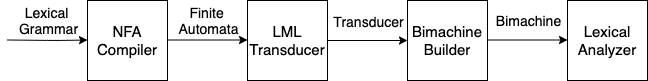
\includegraphics[
		width=14cm,
		keepaspectratio,
	  ]{img/architecture.png}
\end{figure}

В първата част ще представим разширен синтаксис на регулярен израз и разработка на \emph{recursive descent} \hspace*{0cm} парсър, чрез който строим еквивалентния краен автомат. Във втората част ще разгледаме как се строи преобразувател от правила на заместване по стратегията най-ляво-най-дълго срещане и съответно как се строи бимашина по такъв преобразувател. Конструкцията на преобразувателя се съставя изцяло от операции над регулярни езици и релации. В последната част ще видим как се осъществява лексически анализ чрез получената бимашина. Алгоритмите са имплементирани на езика C\#.

\subsection{От регулярен израз към краен автомат}

Регулярните изрази датират още от 50'те години на 20'ти век и са интегрирани в стандартните библиотеки на всички модерни езици за програмиране. Съществуват различни стандарти за представянето им, като тук ще ползваме синтаксис сходен с този на регулярните изрази в Perl. 
На Фигура \ref{fig:RegExSyntax} са представени базовите синтактични единици, чрез които конструираме регулярните изрази.

\begin{figure}[!htb]
	\begin{center}
		\begin{tabular}{ |l|l| } 
		\hline
		Израз & Пояснение \\
		\hline
		\verb/ab/ & конкатенация на символите 'a' и 'b' \\
		\verb/|/ & обединение (\verb/A|B/ - думата се разпознава от \verb/A/ или \verb/B/) \\
		\verb/*/ & 0 или повече срещания (Звезда на Килни) \\
		\verb/+/ & 1 или повече срещания \\
		\verb/?/ & 0 или 1 срещане \\
		\verb/./ & всеки символ от азбуката \\
		\verb/(...)/ & начало и край на група (разпознава израза в скобите) \\
		\verb/[...]/ & множество от символи (\verb/[0-9]/ разпознава цифрите от 0 до 9) \\
		\verb/[^...]/ & отрицание (разпознава символите, които не са в множеството) \\
		\verb/{n}/ & точно n на брой срещания \\
		\verb/{n,}/ & поне n на брой срещания \\
		\verb/{n,m}/ & от n до m на брой срещания \\
		\verb/\/ & буквална интерпретация на символ (\verb/\*/ разпознава '*') \\
		\hline
		\end{tabular}
	\end{center}
	\label{fig:RegExSyntax}
	\caption{Синтаксис на регулярен израз}
\end{figure}

\begin{example}
	Нека разгледаме няколко примерни регулярни израза, демонстриращи представения синтаксис.
	\begin{itemize}
		\item \verb/(a|b)*c/ - разпознава думите, които се състоят от 0 или повече символи 'a' и 'b' и завършват на 'c' като на пример: \emph{ac, bc, abbabac, bbac, c, ...}
		\item \verb/.*true.*/ - думите, които съдържат "true": \emph{abctrue, 1true2_, true, ...}
		\item \verb/[a-zA-Z0-9@]+/ - разпознава думите, които се състоят единствено от латински букви, цифри и '@': \emph{z, 1b@, AbC123, 404, ccC, ...}
		\item \verb/[^ \t\r\n]/ - разпознава всички символи, които не са интервал, табулация или нов ред.
	\end{itemize}
\end{example}

За да построим краен автомат по регулярен израз е нужно първо да дефинираме граматическата му структура. Въвеждаме следната безконтекстна граматика:

\begin{grammar}
	<expr> ::= <term>
	\alt <term> '|' <expr>

	<term> ::= <factor>
	\alt <factor> <term>

	<factor> ::= <atom>
	\alt <atom> <meta-char>
	\alt <atom> '\{' <char-count> '\}'

	<atom> ::= <char>
	\alt '.'
	\alt '(' <expr> ')'
	\alt '[' <char-class> ']'
	\alt '[' '\^{}' <char-class> ']'

	<char-class> ::= <char-class-item> 
	\alt <char-class-item> <char-class>

	<char-class-item> ::= <char> 
	\alt <char> '$-$' <char>

	<char-count> ::= <integer> 
	\alt <integer> ',' 
	\alt <integer> ',' <integer>

	<integer> ::= <digit> 
	\alt <digit> <integer>

	<char> ::= \emph{anyCharExceptMeta}
	\alt '\textbackslash' <any-char>

	<any-char> ::= \emph{alphabet}

	<meta-char> ::= '?' \alt '*' \alt '+'

	<digit> ::= '0' | '1' | \dots | '9'
\end{grammar}

Следвайки тази граматика за всеки коректно дефиниран регулярен израз извличаме дърво на извод, по което чрез обхождане в дълбочина и строим недетерминиран краен автомат. Представяме автоматите и реализираме операциите по между им (конкатенация, обединение, звезда...) спрямо алгоритъма на Томпсън \cite{Thompson:68}. На Фигура \ref{parsetree} е изобразено дърво на извод на регулярен израз спрямо граматиката.

\begin{figure}
	\Tree[.\emph{expr} 
		[.\emph{term} 
		[.\emph{factor} 
			[.\emph{atom} 
				[( [.\emph{expr} 
					[
						[.\emph{term} [.\emph{factor} [.\emph{atom} [.\emph{char} a ]]]] 
						| 
						[.\emph{expr} [.\emph{term} [.\emph{factor} [.\emph{atom} [.\emph{char} b ]]]]  
					]]] 
				) ]]
			[.* ]]
		[.\emph{term}
			[.\emph{factor}
				[.\emph{atom}
					$[$
					[.\emph{char-class}
						[.\emph{char-class-item} [.\emph{char} 0 ] $-$ [.\emph{char} 9 ] ]]
					$]$ ]]]]]
	\label{parsetree}
	\caption{Дърво на извод за регулярния израз \texttt{(a|b)*[0-9]}, който разпознава думите, започващи с нула или повече на брой символи 'a' и 'b', които завършват с цифра, на пример \emph{ab3, bbbb4, 9, aa1, baab4} и т.н. }
\end{figure}

Извличането на дърво на извод по зададен регулярен израз реализираме чрез \emph{парсър за рекурсивно спускане (recursive descent parser)}. Той спада към класа на типа парсъри, които строят дървото на извод \emph{"от горе надолу" (top-down)}, т.е. от корена към листата, започвайки от аксиомата на граматиката (в случая аксиомата е нетерминалът \emph{expr}). Граматическите правила се прилагат от ляво на дясно. Регулярен израз е коректно дефиниран, ако по него може да се построи дърво на извод.

Особеност на \emph{top-down} парсърите е, че работят с ограничен клас от безконтекстни граматики. Ако граматиката съдържа \emph{лява рекурсия}, то е възможно процедурата да изпадне в безкраен цикъл поради факта, че правилата се прилагат от ляво на дясно. Нека разгледаме следния пример за директна рекурсия:

\[ A \to A \alpha \mid \beta \]

Символът \(A\) е нетерминал, докато \( \alpha \) и \( \beta \) са думи, съдържащи терминали и нетерминали, които обаче не започват с \(A\). Тъй като прилагаме правилата от ляво на дясно, то \(A\) ще опита първоначално да изведе \(A\) и така ще изпаднем в безкраен цикъл. Решението тук е да преобразуваме правилото до еквивалентната му дясно-рекурсивна форма.

\[ A \to \beta A' \]
\[ A' \to \alpha A' \mid \epsilon \]

Граматиката на регулярен израз не съдържа лява рекурсия, така че по нея можем  да реализираме \emph{recursive descent} парсър. Идеята е следната:

\begin{itemize}
	\item За всеки нетерминал (\emph{expr, term, factor...}) имплементираме отделен метод.
	\item Построяването на дървото започва с извикването на аксиомата на граматиката (\emph{Expr()}).
	\item Използваме методите \emph{Peek()}, за да видим следващия непрочетен символ от входа и \emph{Eat(char ch)}, който сравнява следващия следващия символ с \emph{ch} и преминава с една позиция напред във входа. \emph{Next()} преминава към следващата позиция във входната дума без значение от символа, т.е. \emph{Eat(Peek())}.
\end{itemize}

Нека разгледаме реализацията на правилото за аксиомата на граматиката.

\begin{grammar}
	<expr> ::= <term>
	\alt <term> '|' <expr>
\end{grammar}

Нетерминалът \emph{expr} има два извода, като и двата започват с нетерминала \emph{term}. След като приложим правилото \emph{term}, проверяваме дали не сме стигнали до края на входа и в случай, че следващият символ е оператора за обединение, то местим входната дума с една позиция, прилагаме правилото \emph{expr} и връщаме обединението на резултатите.

\begin{minted}{csharp}
Fsa Expr() 
{
    var term = Term();
    if (HasMoreChars() && Peek() == '|') {
        Eat('|');
        return term.Union(Expr());
    }
    return term;
}
\end{minted}

Важно е да уточним, че типът \verb/Fsa/ представлява краен автомат т.е. всеки метод, отговарящ на нетерминал в граматиката връща краен автомат. По този начин финалният автомат, съответстващ на регулярния израз се строи директно по време на получаването на дървото на извод. Нека разгледаме метода за нетерминала \emph{char}, който винаги извежда терминален символ, т.е. сме стигнали до листо на дървото.

\begin{minted}{csharp}
Fsa Char() 
{
	if (Peek() == '\') {
		Eat('\');
		var ch = Next();
        if (!alphabet.Contains(ch))
			throw new Exception($"Invalid char {ch}");

      	return FsaBuilder.FromSymbol(ch);
	}
    var ch = Next();
    if (metaChars.Contains(ch))
		throw new Exception($"Unescaped meta symbol {ch}");

    return FsaBuilder.FromSymbol(ch);
}
\end{minted}

Ако сме стингали до символа '\textbackslash', последвалият го символ третираме като буква, независимо дали се използва като оператор. Методът връща автомат, който разпознава единствено прочетения символ. Конвертираме регулярен израз към краен автомат по следния начин:

\begin{minted}{csharp}
	var fsa = new RegExp("(a|b)*c").Automaton;
\end{minted}

\subsection{Конструкция на преобразувател по стратегията най-ляво-най-дълго срещане}

Дефинираме метод, който по зададен краен преобразувател \(T\) и входна азбука, строи преобразувател по стратегията най-ляво-най-дълго срещане. Този метод извежда преобразувател, който е еквивалентен на релацията \( R^{LML}(T) \). Алгоритъмът директно следва конструкцията, представена в глава \ref{sec:LexARegRel}. За целта сме имплементирали базовите алгоритми, реализиращи операциите над крайни автомати и преобразуватели (конкатенация, идентитет, разлика, композиция и пр.) представени в \cite{Mihov:2018}. Реализираме групата от оператори \emph{intro} и \emph{ignore} по Каплан и Кей \cite{Kaplan&Kay:94}.

\begin{minted}{csharp}
static Fst Intro(ISet<char> alphabet, ISet<char> symbols) =>
	FsaBuilder.FromSymbolSet(alphabet.Except(symbols))
		.Identity()
		.Union(
			FsaBuilder.FromEpsilon()
				.Product(FsaBuilder.FromSymbolSet(symbols)))
		.Star();

static Fst IntroX(ISet<char> alphabet, ISet<char> symbols) =>
	Intro(alphabet, symbols)
		.Concat(FsaBuilder.FromSymbolSet(alphabet.Except(symbols)).Identity())
		.Optional();

static Fst Xintro(ISet<char> alphabet, ISet<char> symbols) =>
	FsaBuilder.FromSymbolSet(alphabet.Except(symbols))
		.Identity()
		.Concat(Intro(alphabet, symbols))
		.Optional();

static Fsa Ignore(Fsa fsa, ISet<char> fsaAlphabet, ISet<char> symbols) =>
    fsa.Identity()
		.Compose(Intro(fsaAlphabet, symbols))
		.Range();

static Fsa IgnoreX(Fsa fsa, ISet<char> fsaAlphabet, ISet<char> symbols) =>
	fsa.Identity()
		.Compose(IntroX(fsaAlphabet, symbols))
		.Range();

static Fsa XIgnore(Fsa fsa, ISet<char> fsaAlphabet, ISet<char> symbols) =>
	fsa.Identity()
		.Compose(Xintro(fsaAlphabet, symbols))
		.Range();
\end{minted}

Релацията за задължително заместване \(R^{obl}(T)\) в конктекста на краен преобразувател имплементираме както следва:

\begin{minted}{csharp}
static Fst ToRewriter(this Fst fst, ISet<char> alphabet)
{
	var all = FsaBuilder.FromSymbolSet(alphabet).Star();
	var notInDomain = all
		.Difference(all.Concat(fst.Domain()).Concat(all))
		.Identity()
		.Optional();

	return notInDomain.Concat(fst.Concat(notInDomain).Star());
}
\end{minted}

Вече можем да преминем към имплементацията на преобразувателя, представящ \(R^{LML}(T)\).

\begin{minted}{csharp}
const char cb = '\0';
const char lb = '\u0002';
const char rb = '\u0003';

public static Fst ToLmlRewriter(this Fst fst, ISet<char> alphabet)
{
	if (alphabet.Intersect(markers).Any())
		throw new ArgumentException("The alphabet contains invalid symbols.");

	var alphabetStarFsa = FsaBuilder.FromSymbolSet(alphabet).Star().Minimal();
	var allSymbols = alphabet.Concat(markers).ToHashSet();
	var allSymbolsStarFsa = FsaBuilder.FromSymbolSet(allSymbols).Star().Minimal();

	Fsa NotInLang(Fsa lang) => allSymbolsStarFsa.Difference(lang);
	Fsa ContainsLang(Fsa lang) => allSymbolsStarFsa.Concat(lang, allSymbolsStarFsa);
	Fsa IfPThenS(Fsa p, Fsa s) => NotInLang(p.Concat(NotInLang(s)));
	Fsa IfSThenP(Fsa p, Fsa s) => NotInLang(NotInLang(p).Concat(s));
	Fsa PiffS(Fsa l, Fsa r) => IfPThenS(l, r).Intersect(IfSThenP(l, r));
	Fsa LiffR(Fsa l, Fsa r) => PiffS(allSymbolsStarFsa.Concat(l), r.Concat(allSymbolsStarFsa));
\end{minted}

Първоначално инциализираме автомата, който разпознава думите, съставени от входната азбука (\emph{alphabetStarFsa}) и този, който разпознава думите, съставени от входната азбука и маркерите включително (\emph{allSymbolsStarFsa}) (10-12). В последствие дефинираме операторите над регулярни езици спрямо Каплан и Кей \cite{Kaplan&Kay:94} (14-19).

\begin{minted}[firstnumber=last]{csharp}
	var fstDomain = fst.Domain();
	var initialMatch =
		Intro(allSymbols, new HashSet<char> { cb })
			.Compose(
				LiffR(
					FsaBuilder.FromSymbol(cb),
					XIgnore(fstDomain, allSymbols, new HashSet<char> { cb }))
				.Identity());

	var leftToRight =
		alphabetStarFsa.Identity()
			.Concat(
				FstBuilder.FromWordPair(cb.ToString(), lb.ToString()),
				IgnoreX(fstDomain, allSymbols, new HashSet<char> { cb }).Identity(),
				FstBuilder.FromWordPair(string.Empty, rb.ToString()))
			.Star()
			.Concat(alphabetStarFsa.Identity())
			.Compose(
				FstBuilder.FromWordPair(cb.ToString(), string.Empty).ToRewriter(allSymbols));

	var includesNotLongestMatches =
		ContainsLang(
			FsaBuilder.FromSymbol(lb)
				.Concat(
					IgnoreX(fstDomain, allSymbols, new HashSet<char> { lb, rb })
						.Intersect(ContainsLang(FsaBuilder.FromSymbol(rb)))));
	var longestMatch = NotInLang(includesNotLongestMatches).Identity();

	var replacement =
		FstBuilder.FromWordPair(lb.ToString(), string.Empty)
			.Concat(
				fst,
				FstBuilder.FromWordPair(rb.ToString(), string.Empty))
			.ToRewriter(allSymbols);

	return initialMatch.Compose(leftToRight, longestMatch, replacement);
}
\end{minted}

Строим преобразувателите, съответстващи на релациите \( R^{init}(T) \) (21-27), \(R^{left}(T)\) (29-38), \(R^{long}(T)\) (40-46), \(R^{replace}(T) \) (48-53). Преобразувателят под стратегията най-ляво-най-дълго срещане \(R^{LML}(T)\) получаваме като композираме четири преобразувателя в съответния ред (55).

\subsection{От краен преобразувател към бимашина}

Ако, преобразувателят, построен по стратегията най-ляво-най-дълго срещане е функционален, по него можем да построим еквивалентна в бимашина. Реализираме конструкцията описана в глава \ref{sec:BmConstruct}.

Първата стъпка е да детерминираме подлежащия огледален автомат на входния преобразувател.

\begin{minted}{csharp}
public Bimachine ToBimachine(this Fst rtFst, ISet<char> alphabet)
{
    var fstTransGroupedByTarget = rtFst.Transitions
        .GroupBy(tr => tr.To)
        .ToDictionary(
            g => g.Key, 
            g => g.Select(tr => (In: tr.In, To: tr.From)));

    var rightSStates = new List<ISet<int>> { rtFst.Final.ToHashSet() };
    var rightDfaTrans = new Dictionary<(int From, char Label), int>();

    for (int n = 0; n < rightSStates.Count; n++) {
        var symbolToSStates = rightSStates[n]
            .Where(st => fstTransGroupedByTarget.ContainsKey(st))
            .SelectMany(st => fstTransGroupedByTarget[st])
            .GroupBy(tr => tr.In, tr => tr.To)
            .ToDictionary(g => g.Key, g => g.ToHashSet());

        foreach (var (symbol, subsetState) in symbolToSStates)
            if (!rightSStates.Any(rs => rs.SetEquals(subsetState)))
                rightSStates.Add(subsetState);
        
        foreach (var (label, targetSState) in symbolToSStates)
            rightDfaTrans.Add(
                (n, label.Single()),
                rightSStates.FindIndex(ss => ss.SetEquals(targetSState)));
	}
\end{minted}

На редове 3-7 групираме преходите на подлежащия автомат по състоянията, \textbf{към които}, има преходи. На пример, ако имаме двата прехода \( \langle p_1, a, c, q \rangle \) и \( \langle p_2, b, d, q \rangle \), то ще получим \( \langle q, \{ \langle a, p_1 \rangle, \langle b, p_2 \rangle \} \rangle \). Използвайки тази структура, строим множествата на състоянията и преходите на детерминирания подлежащ огледален автомат (редове 9-29). Тези множества принадлежат на десния автомат на бимашината.

\begin{minted}[firstnumber=last]{csharp}
    var rDfaTransGroupedByTarget = rightDfaTrans
        .GroupBy(kvp => kvp.Value, kvp => (To: kvp.Key.From, Symbol: kvp.Key.Label))
        .ToDictionary(g => g.Key, g => g);

	var fstTransGroupedBySourceAndSymbol = 
		new Dictionary<(char In, int From), ISet<(int To, string Out)>>();

    foreach (var tr in rtFst.Transitions) {
        if (!fstTransGroupedBySourceAndSymbol.ContainsKey((tr.In.Single(), tr.From)))
			fstTransGroupedBySourceAndSymbol[(tr.In.Single(), tr.From)] = 
				new HashSet<(int, string)>();

        fstTransGroupedBySourceAndSymbol[(tr.In.Single(), tr.From)].Add((tr.To, tr.Out));
    }

    var leftDfaStates = new List<(ISet<int> SState, IDictionary<int, int> Selector)>();
    var leftDfaTrans = new Dictionary<(int, char), int>();
    var bmOutput = new Dictionary<(int, char, int), string>();
\end{minted}

Групираме преходите на десния автомат по тяхната дестинация за оптимален досъп (28-30). Аналогично групираме преходите на входния преобразувател по входен символ и състояние (32-41). Инициализираме структурите, в който ще съхраняваме състоянията, преходите на левия автомат, както и изходната функция на бимашината (43-45).

\begin{minted}[firstnumber=last]{csharp}
    var initStateSelector = new Dictionary<int, int>();

    for (int rIndex = 0; rIndex < rightSStates.Count; rIndex++) {
        var initStates = rightSStates[rIndex].Intersect(rtFst.Initial);
        if (initStates.Any())
            initStateSelector.Add(rIndex, initStates.First());
    }

    leftDfaStates.Add((rtFst.Initial.ToHashSet(), initStateSelector));
\end{minted}

Инициализираме \( L_0, \phi_0 \), следвайки директно формалната дефиниция (46-54). Следва да реализираме индукцията, по която строим състоянията и преходите на левия автомат и изходната функция на бимашината.

\begin{minted}[firstnumber=last]{csharp}
    for (int k = 0; k < leftDfaStates.Count; k++) {
        var currLState = leftDfaStates[k];
        var targetLStatesPerSymbol =
            new Dictionary<char, (ISet<int> LSState, IDictionary<int, int> Selector)>();

        foreach (var symbol in alphabet) {
            var targetLSState = new HashSet<int>();

            foreach (var st in currLState.SState)
                if (fstTransGroupedBySourceAndSymbol.ContainsKey((symbol, st)))
                    targetLSState.UnionWith(
                        fstTransGroupedBySourceAndSymbol[(symbol, st)].Select(x => x.To));

			if (!targetLSState.Any()) 
				continue;

            var targetSelector = new Dictionary<int, int>();

            foreach (var (toRIndex, fstState) in currLState.Selector) {
				if (!rDfaTransGroupedByTarget.ContainsKey(toRIndex)) 
					continue;

                foreach (var (fromRIndex, _) in
					rDfaTransGroupedByTarget[toRIndex].Where(p => p.Symbol == symbol)) {

                    if (!fstTransGroupedBySourceAndSymbol.ContainsKey((symbol, fstState)))
                        continue;

                    var reachableFstState = fstTransGroupedBySourceAndSymbol[(symbol, fstState)]
                        .FirstOrDefault(p => rightSStates[fromRIndex].Contains(p.To));

                    if (reachableFstState != default)
                        targetSelector.Add(fromRIndex, reachableFstState.To);
                }
            }

            if (targetSelector.Any())
                targetLStatesPerSymbol.Add(symbol, (targetLSState, targetSelector));
        }

        foreach (var (symbol, (targetLSState, targetSelector)) in targetLStatesPerSymbol) {
            foreach (var (fromRIndex, fstState) in targetSelector) {
                var predecessorOfR = rightDfaTrans[(fromRIndex, symbol)];
                var state = currLState.Selector[predecessorOfR];
                var destinations = fstTransGroupedBySourceAndSymbol[(symbol, state)]
                    .Where(p => p.To == fstState);

                foreach (var (toState, word) in destinations) {
                    var outFnPair = (Key: (k, symbol, fromRIndex), Val: word);

                    if (bmOutput.ContainsKey(outFnPair.Key)) {
                        if (bmOutput[outFnPair.Key] != outFnPair.Val)
                            throw new InvalidOperationException(
								$"Cannot have different values for the same key:" 
									+ "'{bmOutput[outFnPair.Key]}', '{outFnPair.Val}'");
                    }
                    else bmOutput.Add(outFnPair.Key, outFnPair.Val);
                }
            }

            var nextLState = (targetLSState, targetSelector);

            if (!leftDfaStates.Any(ls => AreBmLeftStatesEqual(ls, nextLState)))
                leftDfaStates.Add(nextLState);

            leftDfaTrans.Add(
                (k, symbol),
                leftDfaStates.FindIndex(ls => AreBmLeftStatesEqual(ls, nextLState)));
        }
	}
\end{minted}

Пояснения \dots

\begin{minted}[firstnumber=last]{csharp}
    var leftStateIndices = Enumerable.Range(0, leftDfaStates.Count);
    var leftDfa = new Dfsa(leftStateIndices, 0, Array.Empty<int>(), leftDfaTrans);
    var rightStateIndices = Enumerable.Range(0, rightSStates.Count);
    var rightDfa = new Dfsa(rightStateIndices, 0, Array.Empty<int>(), rightDfaTrans);

    return new Bimachine(leftDfa, rightDfa, bmOutput);
}
\end{minted}

Завършваме конструкцията с представянето на автоматите на бимашината (125-131). Състоянията им бележим с индексите на елементите в съответните множества. Тъй като всяко състояние в тях е финално, не се налага да съхраняваме изрично множество от финални състояния.

\subsection{Лексически анализ чрез бимашина}

В тази част ще съединим сегментите на конструкцията от регулярните изрази до построяването на бимашината, както и ще представим алгоритъм за лексически анализ чрез симулация на бимашина. Крайният резултат е програмен интерфейс, който използваме по следния начин:

\begin{minted}{csharp}
var lexer = Lexer.Create(new[] {
    new Rule("[0-9]+\\.?[0-9]*", "NUM"),
    new Rule("[+*/-]", "OP"),
    new Rule("=", "EQ"),
});
lexer.Input = new InputStream("3.14+1.86=5");

foreach (var token in lexer.GetNextToken())
    Console.WriteLine(token);
\end{minted}

Тази програма ще генерира лексически анализатор, извърши токенизацията на аритметичен израз и изведе следния резултат:

\begin{minted}{text}
[@0,0:3='3.14',<NUM>]
[@1,4:4='+',<OP>]
[@2,5:8='1.86',<NUM>]
[@3,9:9='=',<EQ>]
[@4,10:10='5',<NUM>]
\end{minted}

Разглеждаме процедурата по създаване на лексическия анализатор, следвайки Дефиниция \ref{def:Rlex}

\begin{minted}{csharp}
static Lexer Create(IList<Rule> grammar)
{
	var tokenFsts = new List<Fst>();

	for (int i = 0; i < grammar.Count; i++) {
		var ruleFsa = new RegExp(grammar[i].Pattern).Automaton;
		var ruleFst = FstBuilder.FromWordPair(string.Empty, $"{i}{SoT}")
			.Concat(ruleFsa.Identity())
			.Concat(FstBuilder.FromWordPair(string.Empty, $"{EoT}"));
		tokenFsts.Add(ruleFst);
	}

	var unionFst = tokenFsts.Aggregate((u, f) => u.Union(f));
	var alphabet = unionFst.InputAlphabet
		.Where(s => !string.IsNullOrEmpty(s))
		.Select(s => s.Single())
		.ToHashSet();

	var lmlFst = unionFst.ToLmlRewriter(alphabet);
	var bm = lmlFst.ToBimachine(alphabet);

	return new Lexer(bm, grammar);
}
\end{minted}

 Обхождаме правилата в граматиката и по регулярния израз на всяко строим краен автомат (5-6). В последствие по този автомат получаваме преобразувател, който за всяка дума в езика му ще изведе думата с прикрепяйки индекса на правилото и маркерите за начало и край (7-10). Обединяваме тези преобразуватели и взимаме азбуката по горната лента на получения преобразувател (13-17). От обединението строим преобразувател под стратегията "най-ляво-най-дълго" срещане, който превръщаме в еквивалентната му бимашина (19-20).

\begin{minted}{csharp}
public class Lexer
{
	const char SoT = '\u0002';
	const char EoT = '\u0003';
	readonly IList<Rule> grammar;

	Lexer(Bimachine bm, IList<Rule> grammar) 
	{
        this.Bm = bm;
        this.grammar = grammar;
    }

    public Bimachine Bm { get; }
	public InputStream Input { get; set; }

\end{minted}

Лексическият анализатор съдържа списък от правила (лексическата граматика) и бимашина, построена по съответната граматика. Типът \emph{InputStream} е интерфейс на входния текст, който може да се подаде като низ от символи в паметта или зареди от текстов файл.

% \begin{minted}{csharp}
% class Dfsa
% {
%     public IList<int> States { get; set; }
%     public int Initial { get; set; }
%     public IList<int> Final { get; set; }
%     public IDictionary<(int From, char Label), int>  Transitions { get; set; }
% }
% \end{minted}

% Така представяме детерминиран краен автомат, като функцията на прехода реализираме като двойки ключ-стойност, където ключът е двойка от състояние и символ, а стойността е състоянието, в което попадаме след този преход.

% \begin{minted}{csharp}
% class Bimachine
% {
%     public Dfsa Left { get; set; }
%     public Dfsa Right { get; set; }
%     public IDictionary<(int Lstate, char Symbol, int Rstate), string> 
%         Output { get; private set; }
% }
% \end{minted}

% Аналогично за бимашината имаме два автомата. Left представлява на левия автомат, който сканира текста от ляво на дясно, а Right сканира текста от дясно на ляво. Функцията на изхода са двойки ключ-стойност, където ключът е тройка, състояща се от състояние на левия автомат, входен символ и състояние на десния автомат, а стойността е изведената дума. Вече сме готови да представим метода за токенизация.

\begin{minted}[firstnumber=last]{csharp}
    public IEnumerable<Token> GetNextToken()
    {
        var rPath = Bm.Right.ReverseRecognitionPath(Input);

        if (rPath.Count != Input.Size + 1)
            throw new ArgumentException(
                $"Invalid input symbol. {Input.CharAt(Input.Size - rPath.Count)}");

        var leftState = Bm.Left.Initial;
        var token = new StringBuilder();
        var typeIndex = new StringBuilder();
        var tokenIndex = 0;
        var tokenStartPos = 0;

        for (Input.SetToStart(); !Input.IsExhausted; Input.MoveForward()) {
            var ch = Input.Peek();
            var rightIndex = rPath.Count - 2 - Input.Pos;
            var triple = (leftState, ch, rPath[rightIndex]);

            if (!Bm.Output.ContainsKey(triple))
                throw new ArgumentException($"Invalid token '{token.ToString() + ch}'");

            token.Append(Bm.Output[triple]);

            if (token[token.Length - 1] == EoT)
            {
                token.Remove(token.Length - 1, 1);
                for (var i = 0; token[i] != SoT; i++)
                    typeIndex.Append(token[i]);
                token.Remove(0, typeIndex.Length + 1);

                yield return new Token
                {
                    Index = tokenIndex,
                    Position = (tokenStartPos, Input.Pos),
                    Text = token.ToString(),
                    Type = grammar[int.Parse(typeIndex.ToString())].Name
                };

                token.Clear();
                typeIndex.Clear();
                tokenIndex++;
                tokenStartPos = Input.Pos + 1;
            }

            if (!Bm.Left.Transitions.ContainsKey((leftState, ch)))
                throw new ArgumentException($"Invalid input. {ch}");

            leftState = Bm.Left.Transitions[(leftState, ch)];
        }
    }
}
\end{minted}

Първоначално извличаме редицата от състояния получена от симулацията на десния авомат, прочитайки входния текст от дясно на ляво. Ако автоматът не е прочел целия текст, то входът е невалиден връщаме грешка (17-21). Започваме симулацията на левия автомат, заедно с извеждането на лексемите. Намираме се в началното му състояние (23), променливата \emph{token} (24) изпозваме, за да съхраняваме текста на прочетената лексема, \emph{typeIndex} (25) съдържа индекса на правилото в граматиката, чрез който определяме какъв тип е изведената лексема, \emph{tokenIndex} (26) индикира коя по ред лексема сме извели, а \emph{tokenStartPos} (27) показва на коя позиция в текста започва лексемата. Четем входа от ляво на дясно и на всеки прочетен символ формираме тройката от ляво, дясно състояние и входен символ (30-32). Ако фукнцията на изхода не е дефинирана за тази тройка, връщаме грешка, в противен случай конкатенираме изходната дума към текста, който сме извели до момента (34-37). Ако последният символ на изведената дума е маркер за край на лемсема (end of token), то сме разпознали лексема и преминаваме към извеждането ѝ (39). В този момент \emph{token} е низ, който съдържа едновременно идекса на лексемата и нейната стойност (\verb/<index> SoT <text> EoT/). Елиминираме маркера за край, прочитаме символите от началото докато стигнем до \verb/SoT/, което представлява индекса на правилото, съхраняваме ги в \emph{tokenIndex} и елиминираме сегмента, така че в \emph{token} да остане само текста на лексемата (41-44), докато \emph{tokenIndex} съдържа идекса на правилото в граматиката.  На редове (46-52) извеждаме обект, който съдържа данните на разпознатата лексема - нейният индекс, позиция, текст и тип. Чрез ключовата дума \verb/yield/ указваме, че при следващото извикване на \emph{GetNextToken()}, методът ще продължи изпълнението си, от където е приключил. Подготвяме променливите за разпознаването на следващата лексема (54-57) и продължаваме с итерацията над входния текст, докато не стигнем неговия край, или пък докато левия автомат не може да продължи (60-63), което означава, че текстът съдържа невалидна лексема.

\pagebreak
\begin{thebibliography}{9}
	
	\bibitem{Schutzenberger:61} 
	Schützenberger, M.-P. (1961)
	\textit{A remark on finite transducers.} 
	Information and Control, 4:185–196.

	\bibitem{Kaplan&Kay:94} 
	Kaplan, Ronald and Kay, Martin. (1994)
	\textit{Regular models of phonological rule systems.}
	Computational Linguistics 20(3):331-378

	\bibitem{Karttunen:96}
	Karttunen, Lauri. (1996)
	\textit{Directed Replacement.}
	In Joshi, A. and Palmer, M., editors, Proceedings of the 34th Annual Meeting of the Association for Computational Linguistics, pages 108–115, Santa Cruz.

	\bibitem{Mihov:2018}
	S., Mihov, S., and Schulz, K. U. (2018)
	\textit{Finite-State Techniques Automata, Transducers and Bimachines}
	Chapter 11 "Constructing finite-state devices for text rewriting"

	\bibitem{GerdjikovEtAl:2017}
	Gerdjikov, S., Mihov, S., and Schulz, K. U. (2017)
	\textit{A simple method for building bimachines from functional finite-state transducers.} 
	Carayol, A. and Nicaud, C., editors, Implementation and Application of Automata, pages 113–125. Springer International Publishing.

	\bibitem{Mihov:2018-2}
	S., Mihov, S., and Schulz, K. U. (2018)
	\textit{Finite-State Techniques Automata, Transducers and Bimachines}
	Chapter 6.2 "Equivalence of regular string funcitons and bimachines."

	\bibitem{Thompson:68} 
	Thompson, Ken (1968) 
	\textit{Regular Expression Search Algorithm.} 
	Association for Computing Machinery

\end{thebibliography}	

\end{document}
